
% This LaTeX was auto-generated from an M-file by MATLAB.
% To make changes, update the M-file and republish this document.

\documentclass{article}
\usepackage{graphicx}
\usepackage{color}

\sloppy
\definecolor{lightgray}{gray}{0.5}
\setlength{\parindent}{0pt}

\begin{document}

    
    
\subsection*{Contents}

\begin{itemize}
\setlength{\itemsep}{-1ex}
   \item P1
   \item P2
   \item P3
   \item P4
   \item P5
   \item P6
   \item P7
   \item P8
   \item P9
\end{itemize}


\subsection*{P1}


        \color{lightgray} \begin{verbatim}Warning: To use the default
trust-region-reflective algorithm you must supply
the gradient in the objective function and set
the GradObj option to 'on'. FMINCON will use the
active-set algorithm instead. For information on
applicable algorithms, see Choosing the Algorithm
in the documentation. 
Warning: Your current settings will run a
different algorithm (interior-point) in a future
release. 

Local minimum possible. Constraints satisfied.

fmincon stopped because the predicted change in the objective function
is less than the default value of the function tolerance and constraints 
are satisfied to within the default value of the constraint tolerance.



No active inequalities.
Warning: The specified buffer for
'object_PI/Transport Delay' was too small. During
simulation, the buffer size was temporarily
increased to 5120. In order to generate code, you
need to update the buffer size parameter 
Warning: To use the default
trust-region-reflective algorithm you must supply
the gradient in the objective function and set
the GradObj option to 'on'. FMINCON will use the
active-set algorithm instead. For information on
applicable algorithms, see Choosing the Algorithm
in the documentation. 
Warning: Your current settings will run a
different algorithm (interior-point) in a future
release. 

Local minimum possible. Constraints satisfied.

fmincon stopped because the predicted change in the objective function
is less than the default value of the function tolerance and constraints 
are satisfied to within the default value of the constraint tolerance.



No active inequalities.
\end{verbatim} \color{black}
    
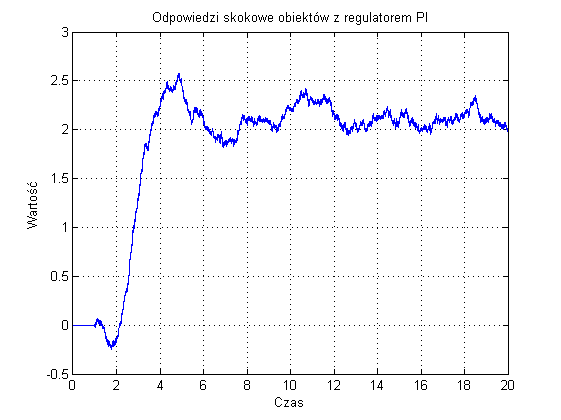
\includegraphics [width=4in]{skrypt_01.png}

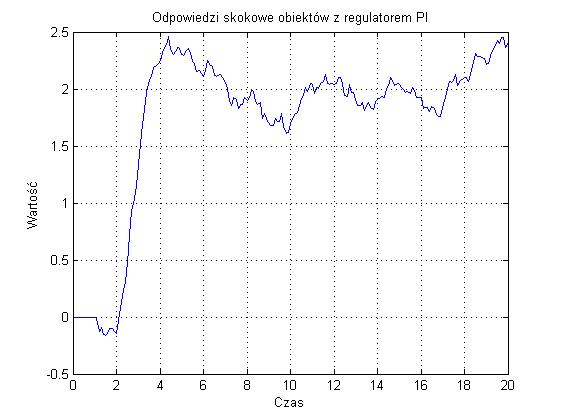
\includegraphics [width=4in]{skrypt_02.png}


\subsection*{P2}


        \color{lightgray} \begin{verbatim}Warning: To use the default
trust-region-reflective algorithm you must supply
the gradient in the objective function and set
the GradObj option to 'on'. FMINCON will use the
active-set algorithm instead. For information on
applicable algorithms, see Choosing the Algorithm
in the documentation. 
Warning: Your current settings will run a
different algorithm (interior-point) in a future
release. 

Local minimum possible. Constraints satisfied.

fmincon stopped because the predicted change in the objective function
is less than the default value of the function tolerance and constraints 
are satisfied to within the default value of the constraint tolerance.



No active inequalities.
Warning: The specified buffer for
'object_PI/Transport Delay' was too small. During
simulation, the buffer size was temporarily
increased to 10240. In order to generate code,
you need to update the buffer size parameter 
Warning: To use the default
trust-region-reflective algorithm you must supply
the gradient in the objective function and set
the GradObj option to 'on'. FMINCON will use the
active-set algorithm instead. For information on
applicable algorithms, see Choosing the Algorithm
in the documentation. 
Warning: Your current settings will run a
different algorithm (interior-point) in a future
release. 

Local minimum possible. Constraints satisfied.

fmincon stopped because the predicted change in the objective function
is less than the default value of the function tolerance and constraints 
are satisfied to within the default value of the constraint tolerance.



No active inequalities.
Warning: The specified buffer for
'object_PI/Transport Delay' was too small. During
simulation, the buffer size was temporarily
increased to 2048. In order to generate code, you
need to update the buffer size parameter 
\end{verbatim} \color{black}
    
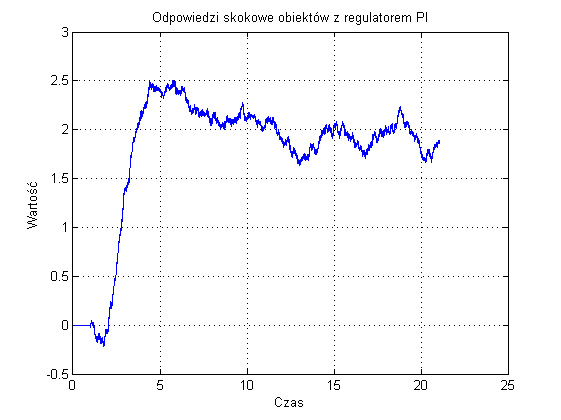
\includegraphics [width=4in]{skrypt_03.png}

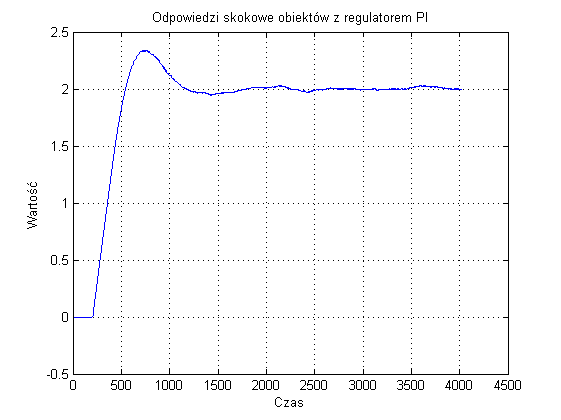
\includegraphics [width=4in]{skrypt_04.png}


\subsection*{P3}


        \color{lightgray} \begin{verbatim}Warning: When delay time is set to zero, the
transport delay block 'single_object/Transport
Delay' is automatically set to support direct
feedthrough. This may cause an algebraic loop. A
Memory Block can be used in place of the
Transport Delay to break the loop 
Warning: To use the default
trust-region-reflective algorithm you must supply
the gradient in the objective function and set
the GradObj option to 'on'. FMINCON will use the
active-set algorithm instead. For information on
applicable algorithms, see Choosing the Algorithm
in the documentation. 
Warning: Your current settings will run a
different algorithm (interior-point) in a future
release. 

Local minimum possible. Constraints satisfied.

fmincon stopped because the predicted change in the objective function
is less than the default value of the function tolerance and constraints 
are satisfied to within the default value of the constraint tolerance.



Active inequalities (to within options.TolCon = 1e-06):
  lower      upper     ineqlin   ineqnonlin
    3                                 
Warning: When delay time is set to zero, the
transport delay block 'single_object/Transport
Delay' is automatically set to support direct
feedthrough. This may cause an algebraic loop. A
Memory Block can be used in place of the
Transport Delay to break the loop 
Warning: To use the default
trust-region-reflective algorithm you must supply
the gradient in the objective function and set
the GradObj option to 'on'. FMINCON will use the
active-set algorithm instead. For information on
applicable algorithms, see Choosing the Algorithm
in the documentation. 
Warning: Your current settings will run a
different algorithm (interior-point) in a future
release. 

Local minimum possible. Constraints satisfied.

fmincon stopped because the predicted change in the objective function
is less than the default value of the function tolerance and constraints 
are satisfied to within the default value of the constraint tolerance.



No active inequalities.
\end{verbatim} \color{black}
    
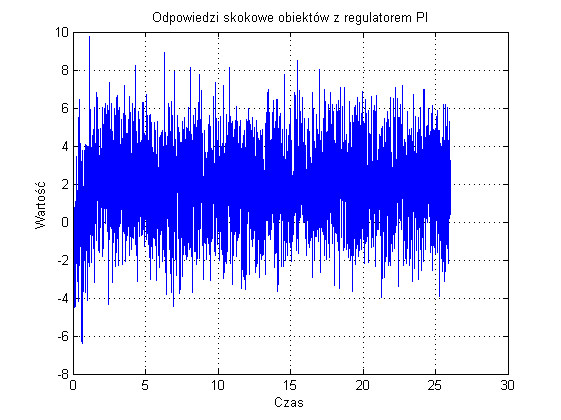
\includegraphics [width=4in]{skrypt_05.png}

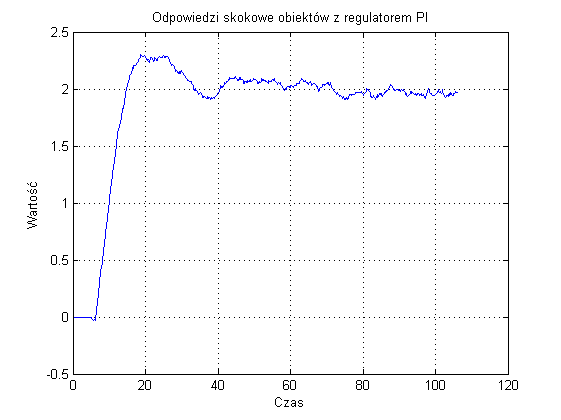
\includegraphics [width=4in]{skrypt_06.png}


\subsection*{P4}


        \color{lightgray} \begin{verbatim}Warning: When delay time is set to zero, the
transport delay block 'single_object/Transport
Delay' is automatically set to support direct
feedthrough. This may cause an algebraic loop. A
Memory Block can be used in place of the
Transport Delay to break the loop 
Warning: To use the default
trust-region-reflective algorithm you must supply
the gradient in the objective function and set
the GradObj option to 'on'. FMINCON will use the
active-set algorithm instead. For information on
applicable algorithms, see Choosing the Algorithm
in the documentation. 
Warning: Your current settings will run a
different algorithm (interior-point) in a future
release. 

Local minimum possible. Constraints satisfied.

fmincon stopped because the predicted change in the objective function
is less than the default value of the function tolerance and constraints 
are satisfied to within the default value of the constraint tolerance.



No active inequalities.
Warning: When delay time is set to zero, the
transport delay block 'single_object/Transport
Delay' is automatically set to support direct
feedthrough. This may cause an algebraic loop. A
Memory Block can be used in place of the
Transport Delay to break the loop 
Warning: To use the default
trust-region-reflective algorithm you must supply
the gradient in the objective function and set
the GradObj option to 'on'. FMINCON will use the
active-set algorithm instead. For information on
applicable algorithms, see Choosing the Algorithm
in the documentation. 
Warning: Your current settings will run a
different algorithm (interior-point) in a future
release. 

Local minimum possible. Constraints satisfied.

fmincon stopped because the predicted change in the objective function
is less than the default value of the function tolerance and constraints 
are satisfied to within the default value of the constraint tolerance.



No active inequalities.
\end{verbatim} \color{black}
    
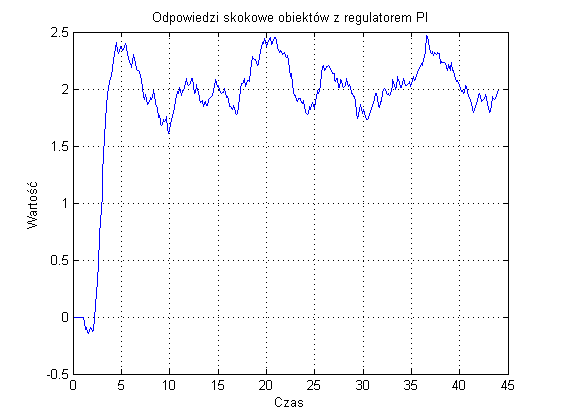
\includegraphics [width=4in]{skrypt_07.png}

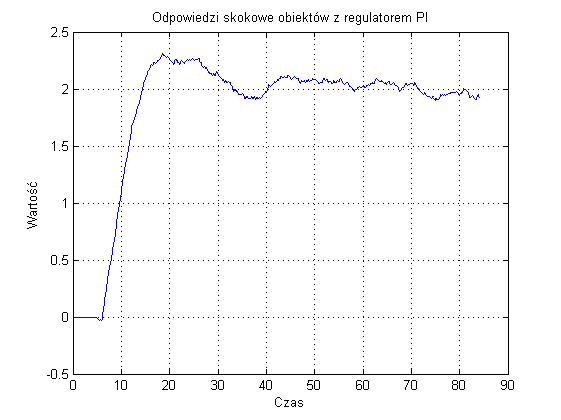
\includegraphics [width=4in]{skrypt_08.png}


\subsection*{P5}


        \color{lightgray} \begin{verbatim}Warning: When delay time is set to zero, the
transport delay block 'single_object/Transport
Delay' is automatically set to support direct
feedthrough. This may cause an algebraic loop. A
Memory Block can be used in place of the
Transport Delay to break the loop 
Warning: To use the default
trust-region-reflective algorithm you must supply
the gradient in the objective function and set
the GradObj option to 'on'. FMINCON will use the
active-set algorithm instead. For information on
applicable algorithms, see Choosing the Algorithm
in the documentation. 
Warning: Your current settings will run a
different algorithm (interior-point) in a future
release. 

Local minimum possible. Constraints satisfied.

fmincon stopped because the predicted change in the objective function
is less than the default value of the function tolerance and constraints 
are satisfied to within the default value of the constraint tolerance.



No active inequalities.
Warning: When delay time is set to zero, the
transport delay block 'single_object/Transport
Delay' is automatically set to support direct
feedthrough. This may cause an algebraic loop. A
Memory Block can be used in place of the
Transport Delay to break the loop 
Warning: The specified simulation stop time
(11.4) is not an integer multiple of the fixed
step size (0.0090000000000000011).  Changing the
stop time to (11.394000000000002).  You can
disable this diagnostic by either specifying a
stop time that is an integer multiple of the
fixed step size, or setting 'Automatic solver
parameter selection' diagnostic to 'none' in the
Diagnostics tab of the Configuration Parameters
dialog 
Warning: To use the default
trust-region-reflective algorithm you must supply
the gradient in the objective function and set
the GradObj option to 'on'. FMINCON will use the
active-set algorithm instead. For information on
applicable algorithms, see Choosing the Algorithm
in the documentation. 
Warning: Your current settings will run a
different algorithm (interior-point) in a future
release. 
Warning: The specified simulation stop time
(11.4) is not an integer multiple of the fixed
step size (0.0090000000000000011).  Changing the
stop time to (11.394000000000002).  You can
disable this diagnostic by either specifying a
stop time that is an integer multiple of the
fixed step size, or setting 'Automatic solver
parameter selection' diagnostic to 'none' in the
Diagnostics tab of the Configuration Parameters
dialog 
Warning: The specified simulation stop time
(11.4) is not an integer multiple of the fixed
step size (0.0090000000000000011).  Changing the
stop time to (11.394000000000002).  You can
disable this diagnostic by either specifying a
stop time that is an integer multiple of the
fixed step size, or setting 'Automatic solver
parameter selection' diagnostic to 'none' in the
Diagnostics tab of the Configuration Parameters
dialog 
Warning: The specified simulation stop time
(11.4) is not an integer multiple of the fixed
step size (0.0090000000000000011).  Changing the
stop time to (11.394000000000002).  You can
disable this diagnostic by either specifying a
stop time that is an integer multiple of the
fixed step size, or setting 'Automatic solver
parameter selection' diagnostic to 'none' in the
Diagnostics tab of the Configuration Parameters
dialog 
Warning: The specified simulation stop time
(11.4) is not an integer multiple of the fixed
step size (0.0090000000000000011).  Changing the
stop time to (11.394000000000002).  You can
disable this diagnostic by either specifying a
stop time that is an integer multiple of the
fixed step size, or setting 'Automatic solver
parameter selection' diagnostic to 'none' in the
Diagnostics tab of the Configuration Parameters
dialog 
Warning: The specified simulation stop time
(11.4) is not an integer multiple of the fixed
step size (0.0090000000000000011).  Changing the
stop time to (11.394000000000002).  You can
disable this diagnostic by either specifying a
stop time that is an integer multiple of the
fixed step size, or setting 'Automatic solver
parameter selection' diagnostic to 'none' in the
Diagnostics tab of the Configuration Parameters
dialog 
Warning: The specified simulation stop time
(11.4) is not an integer multiple of the fixed
step size (0.0090000000000000011).  Changing the
stop time to (11.394000000000002).  You can
disable this diagnostic by either specifying a
stop time that is an integer multiple of the
fixed step size, or setting 'Automatic solver
parameter selection' diagnostic to 'none' in the
Diagnostics tab of the Configuration Parameters
dialog 
Warning: The specified simulation stop time
(11.4) is not an integer multiple of the fixed
step size (0.0090000000000000011).  Changing the
stop time to (11.394000000000002).  You can
disable this diagnostic by either specifying a
stop time that is an integer multiple of the
fixed step size, or setting 'Automatic solver
parameter selection' diagnostic to 'none' in the
Diagnostics tab of the Configuration Parameters
dialog 
Warning: The specified simulation stop time
(11.4) is not an integer multiple of the fixed
step size (0.0090000000000000011).  Changing the
stop time to (11.394000000000002).  You can
disable this diagnostic by either specifying a
stop time that is an integer multiple of the
fixed step size, or setting 'Automatic solver
parameter selection' diagnostic to 'none' in the
Diagnostics tab of the Configuration Parameters
dialog 
Warning: The specified simulation stop time
(11.4) is not an integer multiple of the fixed
step size (0.0090000000000000011).  Changing the
stop time to (11.394000000000002).  You can
disable this diagnostic by either specifying a
stop time that is an integer multiple of the
fixed step size, or setting 'Automatic solver
parameter selection' diagnostic to 'none' in the
Diagnostics tab of the Configuration Parameters
dialog 
Warning: The specified simulation stop time
(11.4) is not an integer multiple of the fixed
step size (0.0090000000000000011).  Changing the
stop time to (11.394000000000002).  You can
disable this diagnostic by either specifying a
stop time that is an integer multiple of the
fixed step size, or setting 'Automatic solver
parameter selection' diagnostic to 'none' in the
Diagnostics tab of the Configuration Parameters
dialog 
Warning: The specified simulation stop time
(11.4) is not an integer multiple of the fixed
step size (0.0090000000000000011).  Changing the
stop time to (11.394000000000002).  You can
disable this diagnostic by either specifying a
stop time that is an integer multiple of the
fixed step size, or setting 'Automatic solver
parameter selection' diagnostic to 'none' in the
Diagnostics tab of the Configuration Parameters
dialog 
Warning: The specified simulation stop time
(11.4) is not an integer multiple of the fixed
step size (0.0090000000000000011).  Changing the
stop time to (11.394000000000002).  You can
disable this diagnostic by either specifying a
stop time that is an integer multiple of the
fixed step size, or setting 'Automatic solver
parameter selection' diagnostic to 'none' in the
Diagnostics tab of the Configuration Parameters
dialog 
Warning: The specified simulation stop time
(11.4) is not an integer multiple of the fixed
step size (0.0090000000000000011).  Changing the
stop time to (11.394000000000002).  You can
disable this diagnostic by either specifying a
stop time that is an integer multiple of the
fixed step size, or setting 'Automatic solver
parameter selection' diagnostic to 'none' in the
Diagnostics tab of the Configuration Parameters
dialog 
Warning: The specified simulation stop time
(11.4) is not an integer multiple of the fixed
step size (0.0090000000000000011).  Changing the
stop time to (11.394000000000002).  You can
disable this diagnostic by either specifying a
stop time that is an integer multiple of the
fixed step size, or setting 'Automatic solver
parameter selection' diagnostic to 'none' in the
Diagnostics tab of the Configuration Parameters
dialog 
Warning: The specified simulation stop time
(11.4) is not an integer multiple of the fixed
step size (0.0090000000000000011).  Changing the
stop time to (11.394000000000002).  You can
disable this diagnostic by either specifying a
stop time that is an integer multiple of the
fixed step size, or setting 'Automatic solver
parameter selection' diagnostic to 'none' in the
Diagnostics tab of the Configuration Parameters
dialog 
Warning: The specified simulation stop time
(11.4) is not an integer multiple of the fixed
step size (0.0090000000000000011).  Changing the
stop time to (11.394000000000002).  You can
disable this diagnostic by either specifying a
stop time that is an integer multiple of the
fixed step size, or setting 'Automatic solver
parameter selection' diagnostic to 'none' in the
Diagnostics tab of the Configuration Parameters
dialog 
Warning: The specified simulation stop time
(11.4) is not an integer multiple of the fixed
step size (0.0090000000000000011).  Changing the
stop time to (11.394000000000002).  You can
disable this diagnostic by either specifying a
stop time that is an integer multiple of the
fixed step size, or setting 'Automatic solver
parameter selection' diagnostic to 'none' in the
Diagnostics tab of the Configuration Parameters
dialog 
Warning: The specified simulation stop time
(11.4) is not an integer multiple of the fixed
step size (0.0090000000000000011).  Changing the
stop time to (11.394000000000002).  You can
disable this diagnostic by either specifying a
stop time that is an integer multiple of the
fixed step size, or setting 'Automatic solver
parameter selection' diagnostic to 'none' in the
Diagnostics tab of the Configuration Parameters
dialog 
Warning: The specified simulation stop time
(11.4) is not an integer multiple of the fixed
step size (0.0090000000000000011).  Changing the
stop time to (11.394000000000002).  You can
disable this diagnostic by either specifying a
stop time that is an integer multiple of the
fixed step size, or setting 'Automatic solver
parameter selection' diagnostic to 'none' in the
Diagnostics tab of the Configuration Parameters
dialog 
Warning: The specified simulation stop time
(11.4) is not an integer multiple of the fixed
step size (0.0090000000000000011).  Changing the
stop time to (11.394000000000002).  You can
disable this diagnostic by either specifying a
stop time that is an integer multiple of the
fixed step size, or setting 'Automatic solver
parameter selection' diagnostic to 'none' in the
Diagnostics tab of the Configuration Parameters
dialog 
Warning: The specified simulation stop time
(11.4) is not an integer multiple of the fixed
step size (0.0090000000000000011).  Changing the
stop time to (11.394000000000002).  You can
disable this diagnostic by either specifying a
stop time that is an integer multiple of the
fixed step size, or setting 'Automatic solver
parameter selection' diagnostic to 'none' in the
Diagnostics tab of the Configuration Parameters
dialog 
Warning: The specified simulation stop time
(11.4) is not an integer multiple of the fixed
step size (0.0090000000000000011).  Changing the
stop time to (11.394000000000002).  You can
disable this diagnostic by either specifying a
stop time that is an integer multiple of the
fixed step size, or setting 'Automatic solver
parameter selection' diagnostic to 'none' in the
Diagnostics tab of the Configuration Parameters
dialog 
Warning: The specified simulation stop time
(11.4) is not an integer multiple of the fixed
step size (0.0090000000000000011).  Changing the
stop time to (11.394000000000002).  You can
disable this diagnostic by either specifying a
stop time that is an integer multiple of the
fixed step size, or setting 'Automatic solver
parameter selection' diagnostic to 'none' in the
Diagnostics tab of the Configuration Parameters
dialog 
Warning: The specified simulation stop time
(11.4) is not an integer multiple of the fixed
step size (0.0090000000000000011).  Changing the
stop time to (11.394000000000002).  You can
disable this diagnostic by either specifying a
stop time that is an integer multiple of the
fixed step size, or setting 'Automatic solver
parameter selection' diagnostic to 'none' in the
Diagnostics tab of the Configuration Parameters
dialog 
Warning: The specified simulation stop time
(11.4) is not an integer multiple of the fixed
step size (0.0090000000000000011).  Changing the
stop time to (11.394000000000002).  You can
disable this diagnostic by either specifying a
stop time that is an integer multiple of the
fixed step size, or setting 'Automatic solver
parameter selection' diagnostic to 'none' in the
Diagnostics tab of the Configuration Parameters
dialog 
Warning: The specified simulation stop time
(11.4) is not an integer multiple of the fixed
step size (0.0090000000000000011).  Changing the
stop time to (11.394000000000002).  You can
disable this diagnostic by either specifying a
stop time that is an integer multiple of the
fixed step size, or setting 'Automatic solver
parameter selection' diagnostic to 'none' in the
Diagnostics tab of the Configuration Parameters
dialog 
Warning: The specified simulation stop time
(11.4) is not an integer multiple of the fixed
step size (0.0090000000000000011).  Changing the
stop time to (11.394000000000002).  You can
disable this diagnostic by either specifying a
stop time that is an integer multiple of the
fixed step size, or setting 'Automatic solver
parameter selection' diagnostic to 'none' in the
Diagnostics tab of the Configuration Parameters
dialog 
Warning: The specified simulation stop time
(11.4) is not an integer multiple of the fixed
step size (0.0090000000000000011).  Changing the
stop time to (11.394000000000002).  You can
disable this diagnostic by either specifying a
stop time that is an integer multiple of the
fixed step size, or setting 'Automatic solver
parameter selection' diagnostic to 'none' in the
Diagnostics tab of the Configuration Parameters
dialog 
Warning: The specified simulation stop time
(11.4) is not an integer multiple of the fixed
step size (0.0090000000000000011).  Changing the
stop time to (11.394000000000002).  You can
disable this diagnostic by either specifying a
stop time that is an integer multiple of the
fixed step size, or setting 'Automatic solver
parameter selection' diagnostic to 'none' in the
Diagnostics tab of the Configuration Parameters
dialog 
Warning: The specified simulation stop time
(11.4) is not an integer multiple of the fixed
step size (0.0090000000000000011).  Changing the
stop time to (11.394000000000002).  You can
disable this diagnostic by either specifying a
stop time that is an integer multiple of the
fixed step size, or setting 'Automatic solver
parameter selection' diagnostic to 'none' in the
Diagnostics tab of the Configuration Parameters
dialog 
Warning: The specified simulation stop time
(11.4) is not an integer multiple of the fixed
step size (0.0090000000000000011).  Changing the
stop time to (11.394000000000002).  You can
disable this diagnostic by either specifying a
stop time that is an integer multiple of the
fixed step size, or setting 'Automatic solver
parameter selection' diagnostic to 'none' in the
Diagnostics tab of the Configuration Parameters
dialog 
Warning: The specified simulation stop time
(11.4) is not an integer multiple of the fixed
step size (0.0090000000000000011).  Changing the
stop time to (11.394000000000002).  You can
disable this diagnostic by either specifying a
stop time that is an integer multiple of the
fixed step size, or setting 'Automatic solver
parameter selection' diagnostic to 'none' in the
Diagnostics tab of the Configuration Parameters
dialog 
Warning: The specified simulation stop time
(11.4) is not an integer multiple of the fixed
step size (0.0090000000000000011).  Changing the
stop time to (11.394000000000002).  You can
disable this diagnostic by either specifying a
stop time that is an integer multiple of the
fixed step size, or setting 'Automatic solver
parameter selection' diagnostic to 'none' in the
Diagnostics tab of the Configuration Parameters
dialog 
Warning: The specified simulation stop time
(11.4) is not an integer multiple of the fixed
step size (0.0090000000000000011).  Changing the
stop time to (11.394000000000002).  You can
disable this diagnostic by either specifying a
stop time that is an integer multiple of the
fixed step size, or setting 'Automatic solver
parameter selection' diagnostic to 'none' in the
Diagnostics tab of the Configuration Parameters
dialog 
Warning: The specified simulation stop time
(11.4) is not an integer multiple of the fixed
step size (0.0090000000000000011).  Changing the
stop time to (11.394000000000002).  You can
disable this diagnostic by either specifying a
stop time that is an integer multiple of the
fixed step size, or setting 'Automatic solver
parameter selection' diagnostic to 'none' in the
Diagnostics tab of the Configuration Parameters
dialog 
Warning: The specified simulation stop time
(11.4) is not an integer multiple of the fixed
step size (0.0090000000000000011).  Changing the
stop time to (11.394000000000002).  You can
disable this diagnostic by either specifying a
stop time that is an integer multiple of the
fixed step size, or setting 'Automatic solver
parameter selection' diagnostic to 'none' in the
Diagnostics tab of the Configuration Parameters
dialog 
Warning: The specified simulation stop time
(11.4) is not an integer multiple of the fixed
step size (0.0090000000000000011).  Changing the
stop time to (11.394000000000002).  You can
disable this diagnostic by either specifying a
stop time that is an integer multiple of the
fixed step size, or setting 'Automatic solver
parameter selection' diagnostic to 'none' in the
Diagnostics tab of the Configuration Parameters
dialog 
Warning: The specified simulation stop time
(11.4) is not an integer multiple of the fixed
step size (0.0090000000000000011).  Changing the
stop time to (11.394000000000002).  You can
disable this diagnostic by either specifying a
stop time that is an integer multiple of the
fixed step size, or setting 'Automatic solver
parameter selection' diagnostic to 'none' in the
Diagnostics tab of the Configuration Parameters
dialog 
Warning: The specified simulation stop time
(11.4) is not an integer multiple of the fixed
step size (0.0090000000000000011).  Changing the
stop time to (11.394000000000002).  You can
disable this diagnostic by either specifying a
stop time that is an integer multiple of the
fixed step size, or setting 'Automatic solver
parameter selection' diagnostic to 'none' in the
Diagnostics tab of the Configuration Parameters
dialog 
Warning: The specified simulation stop time
(11.4) is not an integer multiple of the fixed
step size (0.0090000000000000011).  Changing the
stop time to (11.394000000000002).  You can
disable this diagnostic by either specifying a
stop time that is an integer multiple of the
fixed step size, or setting 'Automatic solver
parameter selection' diagnostic to 'none' in the
Diagnostics tab of the Configuration Parameters
dialog 
Warning: The specified simulation stop time
(11.4) is not an integer multiple of the fixed
step size (0.0090000000000000011).  Changing the
stop time to (11.394000000000002).  You can
disable this diagnostic by either specifying a
stop time that is an integer multiple of the
fixed step size, or setting 'Automatic solver
parameter selection' diagnostic to 'none' in the
Diagnostics tab of the Configuration Parameters
dialog 
Warning: The specified simulation stop time
(11.4) is not an integer multiple of the fixed
step size (0.0090000000000000011).  Changing the
stop time to (11.394000000000002).  You can
disable this diagnostic by either specifying a
stop time that is an integer multiple of the
fixed step size, or setting 'Automatic solver
parameter selection' diagnostic to 'none' in the
Diagnostics tab of the Configuration Parameters
dialog 
Warning: The specified simulation stop time
(11.4) is not an integer multiple of the fixed
step size (0.0090000000000000011).  Changing the
stop time to (11.394000000000002).  You can
disable this diagnostic by either specifying a
stop time that is an integer multiple of the
fixed step size, or setting 'Automatic solver
parameter selection' diagnostic to 'none' in the
Diagnostics tab of the Configuration Parameters
dialog 
Warning: The specified simulation stop time
(11.4) is not an integer multiple of the fixed
step size (0.0090000000000000011).  Changing the
stop time to (11.394000000000002).  You can
disable this diagnostic by either specifying a
stop time that is an integer multiple of the
fixed step size, or setting 'Automatic solver
parameter selection' diagnostic to 'none' in the
Diagnostics tab of the Configuration Parameters
dialog 
Warning: The specified simulation stop time
(11.4) is not an integer multiple of the fixed
step size (0.0090000000000000011).  Changing the
stop time to (11.394000000000002).  You can
disable this diagnostic by either specifying a
stop time that is an integer multiple of the
fixed step size, or setting 'Automatic solver
parameter selection' diagnostic to 'none' in the
Diagnostics tab of the Configuration Parameters
dialog 
Warning: The specified simulation stop time
(11.4) is not an integer multiple of the fixed
step size (0.0090000000000000011).  Changing the
stop time to (11.394000000000002).  You can
disable this diagnostic by either specifying a
stop time that is an integer multiple of the
fixed step size, or setting 'Automatic solver
parameter selection' diagnostic to 'none' in the
Diagnostics tab of the Configuration Parameters
dialog 
Warning: The specified simulation stop time
(11.4) is not an integer multiple of the fixed
step size (0.0090000000000000011).  Changing the
stop time to (11.394000000000002).  You can
disable this diagnostic by either specifying a
stop time that is an integer multiple of the
fixed step size, or setting 'Automatic solver
parameter selection' diagnostic to 'none' in the
Diagnostics tab of the Configuration Parameters
dialog 
Warning: The specified simulation stop time
(11.4) is not an integer multiple of the fixed
step size (0.0090000000000000011).  Changing the
stop time to (11.394000000000002).  You can
disable this diagnostic by either specifying a
stop time that is an integer multiple of the
fixed step size, or setting 'Automatic solver
parameter selection' diagnostic to 'none' in the
Diagnostics tab of the Configuration Parameters
dialog 
Warning: The specified simulation stop time
(11.4) is not an integer multiple of the fixed
step size (0.0090000000000000011).  Changing the
stop time to (11.394000000000002).  You can
disable this diagnostic by either specifying a
stop time that is an integer multiple of the
fixed step size, or setting 'Automatic solver
parameter selection' diagnostic to 'none' in the
Diagnostics tab of the Configuration Parameters
dialog 
Warning: The specified simulation stop time
(11.4) is not an integer multiple of the fixed
step size (0.0090000000000000011).  Changing the
stop time to (11.394000000000002).  You can
disable this diagnostic by either specifying a
stop time that is an integer multiple of the
fixed step size, or setting 'Automatic solver
parameter selection' diagnostic to 'none' in the
Diagnostics tab of the Configuration Parameters
dialog 
Warning: The specified simulation stop time
(11.4) is not an integer multiple of the fixed
step size (0.0090000000000000011).  Changing the
stop time to (11.394000000000002).  You can
disable this diagnostic by either specifying a
stop time that is an integer multiple of the
fixed step size, or setting 'Automatic solver
parameter selection' diagnostic to 'none' in the
Diagnostics tab of the Configuration Parameters
dialog 
Warning: The specified simulation stop time
(11.4) is not an integer multiple of the fixed
step size (0.0090000000000000011).  Changing the
stop time to (11.394000000000002).  You can
disable this diagnostic by either specifying a
stop time that is an integer multiple of the
fixed step size, or setting 'Automatic solver
parameter selection' diagnostic to 'none' in the
Diagnostics tab of the Configuration Parameters
dialog 
Warning: The specified simulation stop time
(11.4) is not an integer multiple of the fixed
step size (0.0090000000000000011).  Changing the
stop time to (11.394000000000002).  You can
disable this diagnostic by either specifying a
stop time that is an integer multiple of the
fixed step size, or setting 'Automatic solver
parameter selection' diagnostic to 'none' in the
Diagnostics tab of the Configuration Parameters
dialog 
Warning: The specified simulation stop time
(11.4) is not an integer multiple of the fixed
step size (0.0090000000000000011).  Changing the
stop time to (11.394000000000002).  You can
disable this diagnostic by either specifying a
stop time that is an integer multiple of the
fixed step size, or setting 'Automatic solver
parameter selection' diagnostic to 'none' in the
Diagnostics tab of the Configuration Parameters
dialog 
Warning: The specified simulation stop time
(11.4) is not an integer multiple of the fixed
step size (0.0090000000000000011).  Changing the
stop time to (11.394000000000002).  You can
disable this diagnostic by either specifying a
stop time that is an integer multiple of the
fixed step size, or setting 'Automatic solver
parameter selection' diagnostic to 'none' in the
Diagnostics tab of the Configuration Parameters
dialog 
Warning: The specified simulation stop time
(11.4) is not an integer multiple of the fixed
step size (0.0090000000000000011).  Changing the
stop time to (11.394000000000002).  You can
disable this diagnostic by either specifying a
stop time that is an integer multiple of the
fixed step size, or setting 'Automatic solver
parameter selection' diagnostic to 'none' in the
Diagnostics tab of the Configuration Parameters
dialog 

Local minimum possible. Constraints satisfied.

fmincon stopped because the predicted change in the objective function
is less than the default value of the function tolerance and constraints 
are satisfied to within the default value of the constraint tolerance.



No active inequalities.
Warning: The specified simulation stop time
(11.4) is not an integer multiple of the fixed
step size (0.0090000000000000011).  Changing the
stop time to (11.394000000000002).  You can
disable this diagnostic by either specifying a
stop time that is an integer multiple of the
fixed step size, or setting 'Automatic solver
parameter selection' diagnostic to 'none' in the
Diagnostics tab of the Configuration Parameters
dialog 
Warning: The specified simulation stop time
(33.2) is not an integer multiple of the fixed
step size (0.0090000000000000011).  Changing the
stop time to (33.192000000000007).  You can
disable this diagnostic by either specifying a
stop time that is an integer multiple of the
fixed step size, or setting 'Automatic solver
parameter selection' diagnostic to 'none' in the
Diagnostics tab of the Configuration Parameters
dialog 
\end{verbatim} \color{black}
    
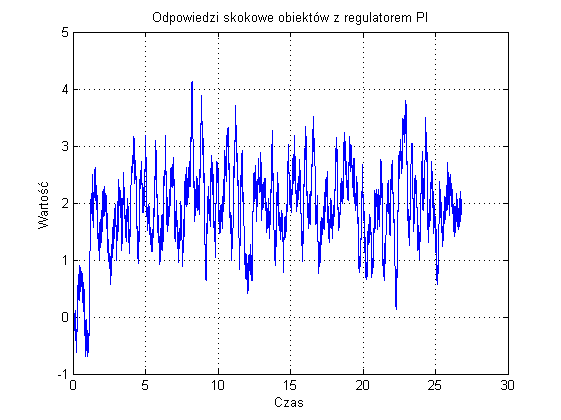
\includegraphics [width=4in]{skrypt_09.png}

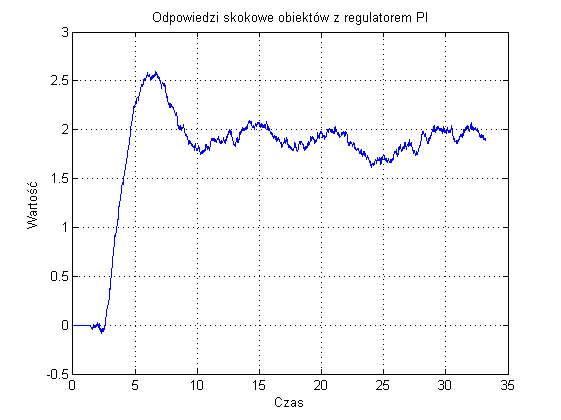
\includegraphics [width=4in]{skrypt_10.png}


\subsection*{P6}


        \color{lightgray} \begin{verbatim}Warning: The specified simulation stop time
(11.94) is not an integer multiple of the fixed
step size (0.0098999999999999991).  Changing the
stop time to (11.9394).  You can disable this
diagnostic by either specifying a stop time that
is an integer multiple of the fixed step size, or
setting 'Automatic solver parameter selection'
diagnostic to 'none' in the Diagnostics tab of
the Configuration Parameters dialog 
Warning: To use the default
trust-region-reflective algorithm you must supply
the gradient in the objective function and set
the GradObj option to 'on'. FMINCON will use the
active-set algorithm instead. For information on
applicable algorithms, see Choosing the Algorithm
in the documentation. 
Warning: Your current settings will run a
different algorithm (interior-point) in a future
release. 
Warning: The specified simulation stop time
(11.94) is not an integer multiple of the fixed
step size (0.0098999999999999991).  Changing the
stop time to (11.9394).  You can disable this
diagnostic by either specifying a stop time that
is an integer multiple of the fixed step size, or
setting 'Automatic solver parameter selection'
diagnostic to 'none' in the Diagnostics tab of
the Configuration Parameters dialog 
Warning: The specified simulation stop time
(11.94) is not an integer multiple of the fixed
step size (0.0098999999999999991).  Changing the
stop time to (11.9394).  You can disable this
diagnostic by either specifying a stop time that
is an integer multiple of the fixed step size, or
setting 'Automatic solver parameter selection'
diagnostic to 'none' in the Diagnostics tab of
the Configuration Parameters dialog 
Warning: The specified simulation stop time
(11.94) is not an integer multiple of the fixed
step size (0.0098999999999999991).  Changing the
stop time to (11.9394).  You can disable this
diagnostic by either specifying a stop time that
is an integer multiple of the fixed step size, or
setting 'Automatic solver parameter selection'
diagnostic to 'none' in the Diagnostics tab of
the Configuration Parameters dialog 
Warning: The specified simulation stop time
(11.94) is not an integer multiple of the fixed
step size (0.0098999999999999991).  Changing the
stop time to (11.9394).  You can disable this
diagnostic by either specifying a stop time that
is an integer multiple of the fixed step size, or
setting 'Automatic solver parameter selection'
diagnostic to 'none' in the Diagnostics tab of
the Configuration Parameters dialog 
Warning: The specified simulation stop time
(11.94) is not an integer multiple of the fixed
step size (0.0098999999999999991).  Changing the
stop time to (11.9394).  You can disable this
diagnostic by either specifying a stop time that
is an integer multiple of the fixed step size, or
setting 'Automatic solver parameter selection'
diagnostic to 'none' in the Diagnostics tab of
the Configuration Parameters dialog 
Warning: The specified simulation stop time
(11.94) is not an integer multiple of the fixed
step size (0.0098999999999999991).  Changing the
stop time to (11.9394).  You can disable this
diagnostic by either specifying a stop time that
is an integer multiple of the fixed step size, or
setting 'Automatic solver parameter selection'
diagnostic to 'none' in the Diagnostics tab of
the Configuration Parameters dialog 
Warning: The specified simulation stop time
(11.94) is not an integer multiple of the fixed
step size (0.0098999999999999991).  Changing the
stop time to (11.9394).  You can disable this
diagnostic by either specifying a stop time that
is an integer multiple of the fixed step size, or
setting 'Automatic solver parameter selection'
diagnostic to 'none' in the Diagnostics tab of
the Configuration Parameters dialog 
Warning: The specified simulation stop time
(11.94) is not an integer multiple of the fixed
step size (0.0098999999999999991).  Changing the
stop time to (11.9394).  You can disable this
diagnostic by either specifying a stop time that
is an integer multiple of the fixed step size, or
setting 'Automatic solver parameter selection'
diagnostic to 'none' in the Diagnostics tab of
the Configuration Parameters dialog 
Warning: The specified simulation stop time
(11.94) is not an integer multiple of the fixed
step size (0.0098999999999999991).  Changing the
stop time to (11.9394).  You can disable this
diagnostic by either specifying a stop time that
is an integer multiple of the fixed step size, or
setting 'Automatic solver parameter selection'
diagnostic to 'none' in the Diagnostics tab of
the Configuration Parameters dialog 
Warning: The specified simulation stop time
(11.94) is not an integer multiple of the fixed
step size (0.0098999999999999991).  Changing the
stop time to (11.9394).  You can disable this
diagnostic by either specifying a stop time that
is an integer multiple of the fixed step size, or
setting 'Automatic solver parameter selection'
diagnostic to 'none' in the Diagnostics tab of
the Configuration Parameters dialog 
Warning: The specified simulation stop time
(11.94) is not an integer multiple of the fixed
step size (0.0098999999999999991).  Changing the
stop time to (11.9394).  You can disable this
diagnostic by either specifying a stop time that
is an integer multiple of the fixed step size, or
setting 'Automatic solver parameter selection'
diagnostic to 'none' in the Diagnostics tab of
the Configuration Parameters dialog 
Warning: The specified simulation stop time
(11.94) is not an integer multiple of the fixed
step size (0.0098999999999999991).  Changing the
stop time to (11.9394).  You can disable this
diagnostic by either specifying a stop time that
is an integer multiple of the fixed step size, or
setting 'Automatic solver parameter selection'
diagnostic to 'none' in the Diagnostics tab of
the Configuration Parameters dialog 
Warning: The specified simulation stop time
(11.94) is not an integer multiple of the fixed
step size (0.0098999999999999991).  Changing the
stop time to (11.9394).  You can disable this
diagnostic by either specifying a stop time that
is an integer multiple of the fixed step size, or
setting 'Automatic solver parameter selection'
diagnostic to 'none' in the Diagnostics tab of
the Configuration Parameters dialog 
Warning: The specified simulation stop time
(11.94) is not an integer multiple of the fixed
step size (0.0098999999999999991).  Changing the
stop time to (11.9394).  You can disable this
diagnostic by either specifying a stop time that
is an integer multiple of the fixed step size, or
setting 'Automatic solver parameter selection'
diagnostic to 'none' in the Diagnostics tab of
the Configuration Parameters dialog 
Warning: The specified simulation stop time
(11.94) is not an integer multiple of the fixed
step size (0.0098999999999999991).  Changing the
stop time to (11.9394).  You can disable this
diagnostic by either specifying a stop time that
is an integer multiple of the fixed step size, or
setting 'Automatic solver parameter selection'
diagnostic to 'none' in the Diagnostics tab of
the Configuration Parameters dialog 
Warning: The specified simulation stop time
(11.94) is not an integer multiple of the fixed
step size (0.0098999999999999991).  Changing the
stop time to (11.9394).  You can disable this
diagnostic by either specifying a stop time that
is an integer multiple of the fixed step size, or
setting 'Automatic solver parameter selection'
diagnostic to 'none' in the Diagnostics tab of
the Configuration Parameters dialog 
Warning: The specified simulation stop time
(11.94) is not an integer multiple of the fixed
step size (0.0098999999999999991).  Changing the
stop time to (11.9394).  You can disable this
diagnostic by either specifying a stop time that
is an integer multiple of the fixed step size, or
setting 'Automatic solver parameter selection'
diagnostic to 'none' in the Diagnostics tab of
the Configuration Parameters dialog 
Warning: The specified simulation stop time
(11.94) is not an integer multiple of the fixed
step size (0.0098999999999999991).  Changing the
stop time to (11.9394).  You can disable this
diagnostic by either specifying a stop time that
is an integer multiple of the fixed step size, or
setting 'Automatic solver parameter selection'
diagnostic to 'none' in the Diagnostics tab of
the Configuration Parameters dialog 
Warning: The specified simulation stop time
(11.94) is not an integer multiple of the fixed
step size (0.0098999999999999991).  Changing the
stop time to (11.9394).  You can disable this
diagnostic by either specifying a stop time that
is an integer multiple of the fixed step size, or
setting 'Automatic solver parameter selection'
diagnostic to 'none' in the Diagnostics tab of
the Configuration Parameters dialog 
Warning: The specified simulation stop time
(11.94) is not an integer multiple of the fixed
step size (0.0098999999999999991).  Changing the
stop time to (11.9394).  You can disable this
diagnostic by either specifying a stop time that
is an integer multiple of the fixed step size, or
setting 'Automatic solver parameter selection'
diagnostic to 'none' in the Diagnostics tab of
the Configuration Parameters dialog 
Warning: The specified simulation stop time
(11.94) is not an integer multiple of the fixed
step size (0.0098999999999999991).  Changing the
stop time to (11.9394).  You can disable this
diagnostic by either specifying a stop time that
is an integer multiple of the fixed step size, or
setting 'Automatic solver parameter selection'
diagnostic to 'none' in the Diagnostics tab of
the Configuration Parameters dialog 
Warning: The specified simulation stop time
(11.94) is not an integer multiple of the fixed
step size (0.0098999999999999991).  Changing the
stop time to (11.9394).  You can disable this
diagnostic by either specifying a stop time that
is an integer multiple of the fixed step size, or
setting 'Automatic solver parameter selection'
diagnostic to 'none' in the Diagnostics tab of
the Configuration Parameters dialog 
Warning: The specified simulation stop time
(11.94) is not an integer multiple of the fixed
step size (0.0098999999999999991).  Changing the
stop time to (11.9394).  You can disable this
diagnostic by either specifying a stop time that
is an integer multiple of the fixed step size, or
setting 'Automatic solver parameter selection'
diagnostic to 'none' in the Diagnostics tab of
the Configuration Parameters dialog 
Warning: The specified simulation stop time
(11.94) is not an integer multiple of the fixed
step size (0.0098999999999999991).  Changing the
stop time to (11.9394).  You can disable this
diagnostic by either specifying a stop time that
is an integer multiple of the fixed step size, or
setting 'Automatic solver parameter selection'
diagnostic to 'none' in the Diagnostics tab of
the Configuration Parameters dialog 
Warning: The specified simulation stop time
(11.94) is not an integer multiple of the fixed
step size (0.0098999999999999991).  Changing the
stop time to (11.9394).  You can disable this
diagnostic by either specifying a stop time that
is an integer multiple of the fixed step size, or
setting 'Automatic solver parameter selection'
diagnostic to 'none' in the Diagnostics tab of
the Configuration Parameters dialog 
Warning: The specified simulation stop time
(11.94) is not an integer multiple of the fixed
step size (0.0098999999999999991).  Changing the
stop time to (11.9394).  You can disable this
diagnostic by either specifying a stop time that
is an integer multiple of the fixed step size, or
setting 'Automatic solver parameter selection'
diagnostic to 'none' in the Diagnostics tab of
the Configuration Parameters dialog 
Warning: The specified simulation stop time
(11.94) is not an integer multiple of the fixed
step size (0.0098999999999999991).  Changing the
stop time to (11.9394).  You can disable this
diagnostic by either specifying a stop time that
is an integer multiple of the fixed step size, or
setting 'Automatic solver parameter selection'
diagnostic to 'none' in the Diagnostics tab of
the Configuration Parameters dialog 
Warning: The specified simulation stop time
(11.94) is not an integer multiple of the fixed
step size (0.0098999999999999991).  Changing the
stop time to (11.9394).  You can disable this
diagnostic by either specifying a stop time that
is an integer multiple of the fixed step size, or
setting 'Automatic solver parameter selection'
diagnostic to 'none' in the Diagnostics tab of
the Configuration Parameters dialog 
Warning: The specified simulation stop time
(11.94) is not an integer multiple of the fixed
step size (0.0098999999999999991).  Changing the
stop time to (11.9394).  You can disable this
diagnostic by either specifying a stop time that
is an integer multiple of the fixed step size, or
setting 'Automatic solver parameter selection'
diagnostic to 'none' in the Diagnostics tab of
the Configuration Parameters dialog 
Warning: The specified simulation stop time
(11.94) is not an integer multiple of the fixed
step size (0.0098999999999999991).  Changing the
stop time to (11.9394).  You can disable this
diagnostic by either specifying a stop time that
is an integer multiple of the fixed step size, or
setting 'Automatic solver parameter selection'
diagnostic to 'none' in the Diagnostics tab of
the Configuration Parameters dialog 
Warning: The specified simulation stop time
(11.94) is not an integer multiple of the fixed
step size (0.0098999999999999991).  Changing the
stop time to (11.9394).  You can disable this
diagnostic by either specifying a stop time that
is an integer multiple of the fixed step size, or
setting 'Automatic solver parameter selection'
diagnostic to 'none' in the Diagnostics tab of
the Configuration Parameters dialog 
Warning: The specified simulation stop time
(11.94) is not an integer multiple of the fixed
step size (0.0098999999999999991).  Changing the
stop time to (11.9394).  You can disable this
diagnostic by either specifying a stop time that
is an integer multiple of the fixed step size, or
setting 'Automatic solver parameter selection'
diagnostic to 'none' in the Diagnostics tab of
the Configuration Parameters dialog 
Warning: The specified simulation stop time
(11.94) is not an integer multiple of the fixed
step size (0.0098999999999999991).  Changing the
stop time to (11.9394).  You can disable this
diagnostic by either specifying a stop time that
is an integer multiple of the fixed step size, or
setting 'Automatic solver parameter selection'
diagnostic to 'none' in the Diagnostics tab of
the Configuration Parameters dialog 
Warning: The specified simulation stop time
(11.94) is not an integer multiple of the fixed
step size (0.0098999999999999991).  Changing the
stop time to (11.9394).  You can disable this
diagnostic by either specifying a stop time that
is an integer multiple of the fixed step size, or
setting 'Automatic solver parameter selection'
diagnostic to 'none' in the Diagnostics tab of
the Configuration Parameters dialog 
Warning: The specified simulation stop time
(11.94) is not an integer multiple of the fixed
step size (0.0098999999999999991).  Changing the
stop time to (11.9394).  You can disable this
diagnostic by either specifying a stop time that
is an integer multiple of the fixed step size, or
setting 'Automatic solver parameter selection'
diagnostic to 'none' in the Diagnostics tab of
the Configuration Parameters dialog 
Warning: The specified simulation stop time
(11.94) is not an integer multiple of the fixed
step size (0.0098999999999999991).  Changing the
stop time to (11.9394).  You can disable this
diagnostic by either specifying a stop time that
is an integer multiple of the fixed step size, or
setting 'Automatic solver parameter selection'
diagnostic to 'none' in the Diagnostics tab of
the Configuration Parameters dialog 
Warning: The specified simulation stop time
(11.94) is not an integer multiple of the fixed
step size (0.0098999999999999991).  Changing the
stop time to (11.9394).  You can disable this
diagnostic by either specifying a stop time that
is an integer multiple of the fixed step size, or
setting 'Automatic solver parameter selection'
diagnostic to 'none' in the Diagnostics tab of
the Configuration Parameters dialog 
Warning: The specified simulation stop time
(11.94) is not an integer multiple of the fixed
step size (0.0098999999999999991).  Changing the
stop time to (11.9394).  You can disable this
diagnostic by either specifying a stop time that
is an integer multiple of the fixed step size, or
setting 'Automatic solver parameter selection'
diagnostic to 'none' in the Diagnostics tab of
the Configuration Parameters dialog 
Warning: The specified simulation stop time
(11.94) is not an integer multiple of the fixed
step size (0.0098999999999999991).  Changing the
stop time to (11.9394).  You can disable this
diagnostic by either specifying a stop time that
is an integer multiple of the fixed step size, or
setting 'Automatic solver parameter selection'
diagnostic to 'none' in the Diagnostics tab of
the Configuration Parameters dialog 
Warning: The specified simulation stop time
(11.94) is not an integer multiple of the fixed
step size (0.0098999999999999991).  Changing the
stop time to (11.9394).  You can disable this
diagnostic by either specifying a stop time that
is an integer multiple of the fixed step size, or
setting 'Automatic solver parameter selection'
diagnostic to 'none' in the Diagnostics tab of
the Configuration Parameters dialog 
Warning: The specified simulation stop time
(11.94) is not an integer multiple of the fixed
step size (0.0098999999999999991).  Changing the
stop time to (11.9394).  You can disable this
diagnostic by either specifying a stop time that
is an integer multiple of the fixed step size, or
setting 'Automatic solver parameter selection'
diagnostic to 'none' in the Diagnostics tab of
the Configuration Parameters dialog 
Warning: The specified simulation stop time
(11.94) is not an integer multiple of the fixed
step size (0.0098999999999999991).  Changing the
stop time to (11.9394).  You can disable this
diagnostic by either specifying a stop time that
is an integer multiple of the fixed step size, or
setting 'Automatic solver parameter selection'
diagnostic to 'none' in the Diagnostics tab of
the Configuration Parameters dialog 
Warning: The specified simulation stop time
(11.94) is not an integer multiple of the fixed
step size (0.0098999999999999991).  Changing the
stop time to (11.9394).  You can disable this
diagnostic by either specifying a stop time that
is an integer multiple of the fixed step size, or
setting 'Automatic solver parameter selection'
diagnostic to 'none' in the Diagnostics tab of
the Configuration Parameters dialog 
Warning: The specified simulation stop time
(11.94) is not an integer multiple of the fixed
step size (0.0098999999999999991).  Changing the
stop time to (11.9394).  You can disable this
diagnostic by either specifying a stop time that
is an integer multiple of the fixed step size, or
setting 'Automatic solver parameter selection'
diagnostic to 'none' in the Diagnostics tab of
the Configuration Parameters dialog 
Warning: The specified simulation stop time
(11.94) is not an integer multiple of the fixed
step size (0.0098999999999999991).  Changing the
stop time to (11.9394).  You can disable this
diagnostic by either specifying a stop time that
is an integer multiple of the fixed step size, or
setting 'Automatic solver parameter selection'
diagnostic to 'none' in the Diagnostics tab of
the Configuration Parameters dialog 
Warning: The specified simulation stop time
(11.94) is not an integer multiple of the fixed
step size (0.0098999999999999991).  Changing the
stop time to (11.9394).  You can disable this
diagnostic by either specifying a stop time that
is an integer multiple of the fixed step size, or
setting 'Automatic solver parameter selection'
diagnostic to 'none' in the Diagnostics tab of
the Configuration Parameters dialog 
Warning: The specified simulation stop time
(11.94) is not an integer multiple of the fixed
step size (0.0098999999999999991).  Changing the
stop time to (11.9394).  You can disable this
diagnostic by either specifying a stop time that
is an integer multiple of the fixed step size, or
setting 'Automatic solver parameter selection'
diagnostic to 'none' in the Diagnostics tab of
the Configuration Parameters dialog 
Warning: The specified simulation stop time
(11.94) is not an integer multiple of the fixed
step size (0.0098999999999999991).  Changing the
stop time to (11.9394).  You can disable this
diagnostic by either specifying a stop time that
is an integer multiple of the fixed step size, or
setting 'Automatic solver parameter selection'
diagnostic to 'none' in the Diagnostics tab of
the Configuration Parameters dialog 
Warning: The specified simulation stop time
(11.94) is not an integer multiple of the fixed
step size (0.0098999999999999991).  Changing the
stop time to (11.9394).  You can disable this
diagnostic by either specifying a stop time that
is an integer multiple of the fixed step size, or
setting 'Automatic solver parameter selection'
diagnostic to 'none' in the Diagnostics tab of
the Configuration Parameters dialog 
Warning: The specified simulation stop time
(11.94) is not an integer multiple of the fixed
step size (0.0098999999999999991).  Changing the
stop time to (11.9394).  You can disable this
diagnostic by either specifying a stop time that
is an integer multiple of the fixed step size, or
setting 'Automatic solver parameter selection'
diagnostic to 'none' in the Diagnostics tab of
the Configuration Parameters dialog 
Warning: The specified simulation stop time
(11.94) is not an integer multiple of the fixed
step size (0.0098999999999999991).  Changing the
stop time to (11.9394).  You can disable this
diagnostic by either specifying a stop time that
is an integer multiple of the fixed step size, or
setting 'Automatic solver parameter selection'
diagnostic to 'none' in the Diagnostics tab of
the Configuration Parameters dialog 
Warning: The specified simulation stop time
(11.94) is not an integer multiple of the fixed
step size (0.0098999999999999991).  Changing the
stop time to (11.9394).  You can disable this
diagnostic by either specifying a stop time that
is an integer multiple of the fixed step size, or
setting 'Automatic solver parameter selection'
diagnostic to 'none' in the Diagnostics tab of
the Configuration Parameters dialog 
Warning: The specified simulation stop time
(11.94) is not an integer multiple of the fixed
step size (0.0098999999999999991).  Changing the
stop time to (11.9394).  You can disable this
diagnostic by either specifying a stop time that
is an integer multiple of the fixed step size, or
setting 'Automatic solver parameter selection'
diagnostic to 'none' in the Diagnostics tab of
the Configuration Parameters dialog 
Warning: The specified simulation stop time
(11.94) is not an integer multiple of the fixed
step size (0.0098999999999999991).  Changing the
stop time to (11.9394).  You can disable this
diagnostic by either specifying a stop time that
is an integer multiple of the fixed step size, or
setting 'Automatic solver parameter selection'
diagnostic to 'none' in the Diagnostics tab of
the Configuration Parameters dialog 
Warning: The specified simulation stop time
(11.94) is not an integer multiple of the fixed
step size (0.0098999999999999991).  Changing the
stop time to (11.9394).  You can disable this
diagnostic by either specifying a stop time that
is an integer multiple of the fixed step size, or
setting 'Automatic solver parameter selection'
diagnostic to 'none' in the Diagnostics tab of
the Configuration Parameters dialog 
Warning: The specified simulation stop time
(11.94) is not an integer multiple of the fixed
step size (0.0098999999999999991).  Changing the
stop time to (11.9394).  You can disable this
diagnostic by either specifying a stop time that
is an integer multiple of the fixed step size, or
setting 'Automatic solver parameter selection'
diagnostic to 'none' in the Diagnostics tab of
the Configuration Parameters dialog 
Warning: The specified simulation stop time
(11.94) is not an integer multiple of the fixed
step size (0.0098999999999999991).  Changing the
stop time to (11.9394).  You can disable this
diagnostic by either specifying a stop time that
is an integer multiple of the fixed step size, or
setting 'Automatic solver parameter selection'
diagnostic to 'none' in the Diagnostics tab of
the Configuration Parameters dialog 
Warning: The specified simulation stop time
(11.94) is not an integer multiple of the fixed
step size (0.0098999999999999991).  Changing the
stop time to (11.9394).  You can disable this
diagnostic by either specifying a stop time that
is an integer multiple of the fixed step size, or
setting 'Automatic solver parameter selection'
diagnostic to 'none' in the Diagnostics tab of
the Configuration Parameters dialog 
Warning: The specified simulation stop time
(11.94) is not an integer multiple of the fixed
step size (0.0098999999999999991).  Changing the
stop time to (11.9394).  You can disable this
diagnostic by either specifying a stop time that
is an integer multiple of the fixed step size, or
setting 'Automatic solver parameter selection'
diagnostic to 'none' in the Diagnostics tab of
the Configuration Parameters dialog 
Warning: The specified simulation stop time
(11.94) is not an integer multiple of the fixed
step size (0.0098999999999999991).  Changing the
stop time to (11.9394).  You can disable this
diagnostic by either specifying a stop time that
is an integer multiple of the fixed step size, or
setting 'Automatic solver parameter selection'
diagnostic to 'none' in the Diagnostics tab of
the Configuration Parameters dialog 
Warning: The specified simulation stop time
(11.94) is not an integer multiple of the fixed
step size (0.0098999999999999991).  Changing the
stop time to (11.9394).  You can disable this
diagnostic by either specifying a stop time that
is an integer multiple of the fixed step size, or
setting 'Automatic solver parameter selection'
diagnostic to 'none' in the Diagnostics tab of
the Configuration Parameters dialog 
Warning: The specified simulation stop time
(11.94) is not an integer multiple of the fixed
step size (0.0098999999999999991).  Changing the
stop time to (11.9394).  You can disable this
diagnostic by either specifying a stop time that
is an integer multiple of the fixed step size, or
setting 'Automatic solver parameter selection'
diagnostic to 'none' in the Diagnostics tab of
the Configuration Parameters dialog 
Warning: The specified simulation stop time
(11.94) is not an integer multiple of the fixed
step size (0.0098999999999999991).  Changing the
stop time to (11.9394).  You can disable this
diagnostic by either specifying a stop time that
is an integer multiple of the fixed step size, or
setting 'Automatic solver parameter selection'
diagnostic to 'none' in the Diagnostics tab of
the Configuration Parameters dialog 
Warning: The specified simulation stop time
(11.94) is not an integer multiple of the fixed
step size (0.0098999999999999991).  Changing the
stop time to (11.9394).  You can disable this
diagnostic by either specifying a stop time that
is an integer multiple of the fixed step size, or
setting 'Automatic solver parameter selection'
diagnostic to 'none' in the Diagnostics tab of
the Configuration Parameters dialog 
Warning: The specified simulation stop time
(11.94) is not an integer multiple of the fixed
step size (0.0098999999999999991).  Changing the
stop time to (11.9394).  You can disable this
diagnostic by either specifying a stop time that
is an integer multiple of the fixed step size, or
setting 'Automatic solver parameter selection'
diagnostic to 'none' in the Diagnostics tab of
the Configuration Parameters dialog 
Warning: The specified simulation stop time
(11.94) is not an integer multiple of the fixed
step size (0.0098999999999999991).  Changing the
stop time to (11.9394).  You can disable this
diagnostic by either specifying a stop time that
is an integer multiple of the fixed step size, or
setting 'Automatic solver parameter selection'
diagnostic to 'none' in the Diagnostics tab of
the Configuration Parameters dialog 
Warning: The specified simulation stop time
(11.94) is not an integer multiple of the fixed
step size (0.0098999999999999991).  Changing the
stop time to (11.9394).  You can disable this
diagnostic by either specifying a stop time that
is an integer multiple of the fixed step size, or
setting 'Automatic solver parameter selection'
diagnostic to 'none' in the Diagnostics tab of
the Configuration Parameters dialog 
Warning: The specified simulation stop time
(11.94) is not an integer multiple of the fixed
step size (0.0098999999999999991).  Changing the
stop time to (11.9394).  You can disable this
diagnostic by either specifying a stop time that
is an integer multiple of the fixed step size, or
setting 'Automatic solver parameter selection'
diagnostic to 'none' in the Diagnostics tab of
the Configuration Parameters dialog 
Warning: The specified simulation stop time
(11.94) is not an integer multiple of the fixed
step size (0.0098999999999999991).  Changing the
stop time to (11.9394).  You can disable this
diagnostic by either specifying a stop time that
is an integer multiple of the fixed step size, or
setting 'Automatic solver parameter selection'
diagnostic to 'none' in the Diagnostics tab of
the Configuration Parameters dialog 
Warning: The specified simulation stop time
(11.94) is not an integer multiple of the fixed
step size (0.0098999999999999991).  Changing the
stop time to (11.9394).  You can disable this
diagnostic by either specifying a stop time that
is an integer multiple of the fixed step size, or
setting 'Automatic solver parameter selection'
diagnostic to 'none' in the Diagnostics tab of
the Configuration Parameters dialog 
Warning: The specified simulation stop time
(11.94) is not an integer multiple of the fixed
step size (0.0098999999999999991).  Changing the
stop time to (11.9394).  You can disable this
diagnostic by either specifying a stop time that
is an integer multiple of the fixed step size, or
setting 'Automatic solver parameter selection'
diagnostic to 'none' in the Diagnostics tab of
the Configuration Parameters dialog 
Warning: The specified simulation stop time
(11.94) is not an integer multiple of the fixed
step size (0.0098999999999999991).  Changing the
stop time to (11.9394).  You can disable this
diagnostic by either specifying a stop time that
is an integer multiple of the fixed step size, or
setting 'Automatic solver parameter selection'
diagnostic to 'none' in the Diagnostics tab of
the Configuration Parameters dialog 
Warning: The specified simulation stop time
(11.94) is not an integer multiple of the fixed
step size (0.0098999999999999991).  Changing the
stop time to (11.9394).  You can disable this
diagnostic by either specifying a stop time that
is an integer multiple of the fixed step size, or
setting 'Automatic solver parameter selection'
diagnostic to 'none' in the Diagnostics tab of
the Configuration Parameters dialog 
Warning: The specified simulation stop time
(11.94) is not an integer multiple of the fixed
step size (0.0098999999999999991).  Changing the
stop time to (11.9394).  You can disable this
diagnostic by either specifying a stop time that
is an integer multiple of the fixed step size, or
setting 'Automatic solver parameter selection'
diagnostic to 'none' in the Diagnostics tab of
the Configuration Parameters dialog 
Warning: The specified simulation stop time
(11.94) is not an integer multiple of the fixed
step size (0.0098999999999999991).  Changing the
stop time to (11.9394).  You can disable this
diagnostic by either specifying a stop time that
is an integer multiple of the fixed step size, or
setting 'Automatic solver parameter selection'
diagnostic to 'none' in the Diagnostics tab of
the Configuration Parameters dialog 
Warning: The specified simulation stop time
(11.94) is not an integer multiple of the fixed
step size (0.0098999999999999991).  Changing the
stop time to (11.9394).  You can disable this
diagnostic by either specifying a stop time that
is an integer multiple of the fixed step size, or
setting 'Automatic solver parameter selection'
diagnostic to 'none' in the Diagnostics tab of
the Configuration Parameters dialog 
Warning: The specified simulation stop time
(11.94) is not an integer multiple of the fixed
step size (0.0098999999999999991).  Changing the
stop time to (11.9394).  You can disable this
diagnostic by either specifying a stop time that
is an integer multiple of the fixed step size, or
setting 'Automatic solver parameter selection'
diagnostic to 'none' in the Diagnostics tab of
the Configuration Parameters dialog 
Warning: The specified simulation stop time
(11.94) is not an integer multiple of the fixed
step size (0.0098999999999999991).  Changing the
stop time to (11.9394).  You can disable this
diagnostic by either specifying a stop time that
is an integer multiple of the fixed step size, or
setting 'Automatic solver parameter selection'
diagnostic to 'none' in the Diagnostics tab of
the Configuration Parameters dialog 
Warning: The specified simulation stop time
(11.94) is not an integer multiple of the fixed
step size (0.0098999999999999991).  Changing the
stop time to (11.9394).  You can disable this
diagnostic by either specifying a stop time that
is an integer multiple of the fixed step size, or
setting 'Automatic solver parameter selection'
diagnostic to 'none' in the Diagnostics tab of
the Configuration Parameters dialog 
Warning: The specified simulation stop time
(11.94) is not an integer multiple of the fixed
step size (0.0098999999999999991).  Changing the
stop time to (11.9394).  You can disable this
diagnostic by either specifying a stop time that
is an integer multiple of the fixed step size, or
setting 'Automatic solver parameter selection'
diagnostic to 'none' in the Diagnostics tab of
the Configuration Parameters dialog 
Warning: The specified simulation stop time
(11.94) is not an integer multiple of the fixed
step size (0.0098999999999999991).  Changing the
stop time to (11.9394).  You can disable this
diagnostic by either specifying a stop time that
is an integer multiple of the fixed step size, or
setting 'Automatic solver parameter selection'
diagnostic to 'none' in the Diagnostics tab of
the Configuration Parameters dialog 
Warning: The specified simulation stop time
(11.94) is not an integer multiple of the fixed
step size (0.0098999999999999991).  Changing the
stop time to (11.9394).  You can disable this
diagnostic by either specifying a stop time that
is an integer multiple of the fixed step size, or
setting 'Automatic solver parameter selection'
diagnostic to 'none' in the Diagnostics tab of
the Configuration Parameters dialog 
Warning: The specified simulation stop time
(11.94) is not an integer multiple of the fixed
step size (0.0098999999999999991).  Changing the
stop time to (11.9394).  You can disable this
diagnostic by either specifying a stop time that
is an integer multiple of the fixed step size, or
setting 'Automatic solver parameter selection'
diagnostic to 'none' in the Diagnostics tab of
the Configuration Parameters dialog 
Warning: The specified simulation stop time
(11.94) is not an integer multiple of the fixed
step size (0.0098999999999999991).  Changing the
stop time to (11.9394).  You can disable this
diagnostic by either specifying a stop time that
is an integer multiple of the fixed step size, or
setting 'Automatic solver parameter selection'
diagnostic to 'none' in the Diagnostics tab of
the Configuration Parameters dialog 
Warning: The specified simulation stop time
(11.94) is not an integer multiple of the fixed
step size (0.0098999999999999991).  Changing the
stop time to (11.9394).  You can disable this
diagnostic by either specifying a stop time that
is an integer multiple of the fixed step size, or
setting 'Automatic solver parameter selection'
diagnostic to 'none' in the Diagnostics tab of
the Configuration Parameters dialog 
Warning: The specified simulation stop time
(11.94) is not an integer multiple of the fixed
step size (0.0098999999999999991).  Changing the
stop time to (11.9394).  You can disable this
diagnostic by either specifying a stop time that
is an integer multiple of the fixed step size, or
setting 'Automatic solver parameter selection'
diagnostic to 'none' in the Diagnostics tab of
the Configuration Parameters dialog 
Warning: The specified simulation stop time
(11.94) is not an integer multiple of the fixed
step size (0.0098999999999999991).  Changing the
stop time to (11.9394).  You can disable this
diagnostic by either specifying a stop time that
is an integer multiple of the fixed step size, or
setting 'Automatic solver parameter selection'
diagnostic to 'none' in the Diagnostics tab of
the Configuration Parameters dialog 
Warning: The specified simulation stop time
(11.94) is not an integer multiple of the fixed
step size (0.0098999999999999991).  Changing the
stop time to (11.9394).  You can disable this
diagnostic by either specifying a stop time that
is an integer multiple of the fixed step size, or
setting 'Automatic solver parameter selection'
diagnostic to 'none' in the Diagnostics tab of
the Configuration Parameters dialog 
Warning: The specified simulation stop time
(11.94) is not an integer multiple of the fixed
step size (0.0098999999999999991).  Changing the
stop time to (11.9394).  You can disable this
diagnostic by either specifying a stop time that
is an integer multiple of the fixed step size, or
setting 'Automatic solver parameter selection'
diagnostic to 'none' in the Diagnostics tab of
the Configuration Parameters dialog 
Warning: The specified simulation stop time
(11.94) is not an integer multiple of the fixed
step size (0.0098999999999999991).  Changing the
stop time to (11.9394).  You can disable this
diagnostic by either specifying a stop time that
is an integer multiple of the fixed step size, or
setting 'Automatic solver parameter selection'
diagnostic to 'none' in the Diagnostics tab of
the Configuration Parameters dialog 
Warning: The specified simulation stop time
(11.94) is not an integer multiple of the fixed
step size (0.0098999999999999991).  Changing the
stop time to (11.9394).  You can disable this
diagnostic by either specifying a stop time that
is an integer multiple of the fixed step size, or
setting 'Automatic solver parameter selection'
diagnostic to 'none' in the Diagnostics tab of
the Configuration Parameters dialog 
Warning: The specified simulation stop time
(11.94) is not an integer multiple of the fixed
step size (0.0098999999999999991).  Changing the
stop time to (11.9394).  You can disable this
diagnostic by either specifying a stop time that
is an integer multiple of the fixed step size, or
setting 'Automatic solver parameter selection'
diagnostic to 'none' in the Diagnostics tab of
the Configuration Parameters dialog 
Warning: The specified simulation stop time
(11.94) is not an integer multiple of the fixed
step size (0.0098999999999999991).  Changing the
stop time to (11.9394).  You can disable this
diagnostic by either specifying a stop time that
is an integer multiple of the fixed step size, or
setting 'Automatic solver parameter selection'
diagnostic to 'none' in the Diagnostics tab of
the Configuration Parameters dialog 
Warning: The specified simulation stop time
(11.94) is not an integer multiple of the fixed
step size (0.0098999999999999991).  Changing the
stop time to (11.9394).  You can disable this
diagnostic by either specifying a stop time that
is an integer multiple of the fixed step size, or
setting 'Automatic solver parameter selection'
diagnostic to 'none' in the Diagnostics tab of
the Configuration Parameters dialog 
Warning: The specified simulation stop time
(11.94) is not an integer multiple of the fixed
step size (0.0098999999999999991).  Changing the
stop time to (11.9394).  You can disable this
diagnostic by either specifying a stop time that
is an integer multiple of the fixed step size, or
setting 'Automatic solver parameter selection'
diagnostic to 'none' in the Diagnostics tab of
the Configuration Parameters dialog 
Warning: The specified simulation stop time
(11.94) is not an integer multiple of the fixed
step size (0.0098999999999999991).  Changing the
stop time to (11.9394).  You can disable this
diagnostic by either specifying a stop time that
is an integer multiple of the fixed step size, or
setting 'Automatic solver parameter selection'
diagnostic to 'none' in the Diagnostics tab of
the Configuration Parameters dialog 
Warning: The specified simulation stop time
(11.94) is not an integer multiple of the fixed
step size (0.0098999999999999991).  Changing the
stop time to (11.9394).  You can disable this
diagnostic by either specifying a stop time that
is an integer multiple of the fixed step size, or
setting 'Automatic solver parameter selection'
diagnostic to 'none' in the Diagnostics tab of
the Configuration Parameters dialog 
Warning: The specified simulation stop time
(11.94) is not an integer multiple of the fixed
step size (0.0098999999999999991).  Changing the
stop time to (11.9394).  You can disable this
diagnostic by either specifying a stop time that
is an integer multiple of the fixed step size, or
setting 'Automatic solver parameter selection'
diagnostic to 'none' in the Diagnostics tab of
the Configuration Parameters dialog 
Warning: The specified simulation stop time
(11.94) is not an integer multiple of the fixed
step size (0.0098999999999999991).  Changing the
stop time to (11.9394).  You can disable this
diagnostic by either specifying a stop time that
is an integer multiple of the fixed step size, or
setting 'Automatic solver parameter selection'
diagnostic to 'none' in the Diagnostics tab of
the Configuration Parameters dialog 
Warning: The specified simulation stop time
(11.94) is not an integer multiple of the fixed
step size (0.0098999999999999991).  Changing the
stop time to (11.9394).  You can disable this
diagnostic by either specifying a stop time that
is an integer multiple of the fixed step size, or
setting 'Automatic solver parameter selection'
diagnostic to 'none' in the Diagnostics tab of
the Configuration Parameters dialog 
Warning: The specified simulation stop time
(11.94) is not an integer multiple of the fixed
step size (0.0098999999999999991).  Changing the
stop time to (11.9394).  You can disable this
diagnostic by either specifying a stop time that
is an integer multiple of the fixed step size, or
setting 'Automatic solver parameter selection'
diagnostic to 'none' in the Diagnostics tab of
the Configuration Parameters dialog 
Warning: The specified simulation stop time
(11.94) is not an integer multiple of the fixed
step size (0.0098999999999999991).  Changing the
stop time to (11.9394).  You can disable this
diagnostic by either specifying a stop time that
is an integer multiple of the fixed step size, or
setting 'Automatic solver parameter selection'
diagnostic to 'none' in the Diagnostics tab of
the Configuration Parameters dialog 
Warning: The specified simulation stop time
(11.94) is not an integer multiple of the fixed
step size (0.0098999999999999991).  Changing the
stop time to (11.9394).  You can disable this
diagnostic by either specifying a stop time that
is an integer multiple of the fixed step size, or
setting 'Automatic solver parameter selection'
diagnostic to 'none' in the Diagnostics tab of
the Configuration Parameters dialog 
Warning: The specified simulation stop time
(11.94) is not an integer multiple of the fixed
step size (0.0098999999999999991).  Changing the
stop time to (11.9394).  You can disable this
diagnostic by either specifying a stop time that
is an integer multiple of the fixed step size, or
setting 'Automatic solver parameter selection'
diagnostic to 'none' in the Diagnostics tab of
the Configuration Parameters dialog 
Warning: The specified simulation stop time
(11.94) is not an integer multiple of the fixed
step size (0.0098999999999999991).  Changing the
stop time to (11.9394).  You can disable this
diagnostic by either specifying a stop time that
is an integer multiple of the fixed step size, or
setting 'Automatic solver parameter selection'
diagnostic to 'none' in the Diagnostics tab of
the Configuration Parameters dialog 
Warning: The specified simulation stop time
(11.94) is not an integer multiple of the fixed
step size (0.0098999999999999991).  Changing the
stop time to (11.9394).  You can disable this
diagnostic by either specifying a stop time that
is an integer multiple of the fixed step size, or
setting 'Automatic solver parameter selection'
diagnostic to 'none' in the Diagnostics tab of
the Configuration Parameters dialog 
Warning: The specified simulation stop time
(11.94) is not an integer multiple of the fixed
step size (0.0098999999999999991).  Changing the
stop time to (11.9394).  You can disable this
diagnostic by either specifying a stop time that
is an integer multiple of the fixed step size, or
setting 'Automatic solver parameter selection'
diagnostic to 'none' in the Diagnostics tab of
the Configuration Parameters dialog 
Warning: The specified simulation stop time
(11.94) is not an integer multiple of the fixed
step size (0.0098999999999999991).  Changing the
stop time to (11.9394).  You can disable this
diagnostic by either specifying a stop time that
is an integer multiple of the fixed step size, or
setting 'Automatic solver parameter selection'
diagnostic to 'none' in the Diagnostics tab of
the Configuration Parameters dialog 
Warning: The specified simulation stop time
(11.94) is not an integer multiple of the fixed
step size (0.0098999999999999991).  Changing the
stop time to (11.9394).  You can disable this
diagnostic by either specifying a stop time that
is an integer multiple of the fixed step size, or
setting 'Automatic solver parameter selection'
diagnostic to 'none' in the Diagnostics tab of
the Configuration Parameters dialog 
Warning: The specified simulation stop time
(11.94) is not an integer multiple of the fixed
step size (0.0098999999999999991).  Changing the
stop time to (11.9394).  You can disable this
diagnostic by either specifying a stop time that
is an integer multiple of the fixed step size, or
setting 'Automatic solver parameter selection'
diagnostic to 'none' in the Diagnostics tab of
the Configuration Parameters dialog 
Warning: The specified simulation stop time
(11.94) is not an integer multiple of the fixed
step size (0.0098999999999999991).  Changing the
stop time to (11.9394).  You can disable this
diagnostic by either specifying a stop time that
is an integer multiple of the fixed step size, or
setting 'Automatic solver parameter selection'
diagnostic to 'none' in the Diagnostics tab of
the Configuration Parameters dialog 
Warning: The specified simulation stop time
(11.94) is not an integer multiple of the fixed
step size (0.0098999999999999991).  Changing the
stop time to (11.9394).  You can disable this
diagnostic by either specifying a stop time that
is an integer multiple of the fixed step size, or
setting 'Automatic solver parameter selection'
diagnostic to 'none' in the Diagnostics tab of
the Configuration Parameters dialog 
Warning: The specified simulation stop time
(11.94) is not an integer multiple of the fixed
step size (0.0098999999999999991).  Changing the
stop time to (11.9394).  You can disable this
diagnostic by either specifying a stop time that
is an integer multiple of the fixed step size, or
setting 'Automatic solver parameter selection'
diagnostic to 'none' in the Diagnostics tab of
the Configuration Parameters dialog 
Warning: The specified simulation stop time
(11.94) is not an integer multiple of the fixed
step size (0.0098999999999999991).  Changing the
stop time to (11.9394).  You can disable this
diagnostic by either specifying a stop time that
is an integer multiple of the fixed step size, or
setting 'Automatic solver parameter selection'
diagnostic to 'none' in the Diagnostics tab of
the Configuration Parameters dialog 
Warning: The specified simulation stop time
(11.94) is not an integer multiple of the fixed
step size (0.0098999999999999991).  Changing the
stop time to (11.9394).  You can disable this
diagnostic by either specifying a stop time that
is an integer multiple of the fixed step size, or
setting 'Automatic solver parameter selection'
diagnostic to 'none' in the Diagnostics tab of
the Configuration Parameters dialog 
Warning: The specified simulation stop time
(11.94) is not an integer multiple of the fixed
step size (0.0098999999999999991).  Changing the
stop time to (11.9394).  You can disable this
diagnostic by either specifying a stop time that
is an integer multiple of the fixed step size, or
setting 'Automatic solver parameter selection'
diagnostic to 'none' in the Diagnostics tab of
the Configuration Parameters dialog 
Warning: The specified simulation stop time
(11.94) is not an integer multiple of the fixed
step size (0.0098999999999999991).  Changing the
stop time to (11.9394).  You can disable this
diagnostic by either specifying a stop time that
is an integer multiple of the fixed step size, or
setting 'Automatic solver parameter selection'
diagnostic to 'none' in the Diagnostics tab of
the Configuration Parameters dialog 
Warning: The specified simulation stop time
(11.94) is not an integer multiple of the fixed
step size (0.0098999999999999991).  Changing the
stop time to (11.9394).  You can disable this
diagnostic by either specifying a stop time that
is an integer multiple of the fixed step size, or
setting 'Automatic solver parameter selection'
diagnostic to 'none' in the Diagnostics tab of
the Configuration Parameters dialog 
Warning: The specified simulation stop time
(11.94) is not an integer multiple of the fixed
step size (0.0098999999999999991).  Changing the
stop time to (11.9394).  You can disable this
diagnostic by either specifying a stop time that
is an integer multiple of the fixed step size, or
setting 'Automatic solver parameter selection'
diagnostic to 'none' in the Diagnostics tab of
the Configuration Parameters dialog 
Warning: The specified simulation stop time
(11.94) is not an integer multiple of the fixed
step size (0.0098999999999999991).  Changing the
stop time to (11.9394).  You can disable this
diagnostic by either specifying a stop time that
is an integer multiple of the fixed step size, or
setting 'Automatic solver parameter selection'
diagnostic to 'none' in the Diagnostics tab of
the Configuration Parameters dialog 
Warning: The specified simulation stop time
(11.94) is not an integer multiple of the fixed
step size (0.0098999999999999991).  Changing the
stop time to (11.9394).  You can disable this
diagnostic by either specifying a stop time that
is an integer multiple of the fixed step size, or
setting 'Automatic solver parameter selection'
diagnostic to 'none' in the Diagnostics tab of
the Configuration Parameters dialog 
Warning: The specified simulation stop time
(11.94) is not an integer multiple of the fixed
step size (0.0098999999999999991).  Changing the
stop time to (11.9394).  You can disable this
diagnostic by either specifying a stop time that
is an integer multiple of the fixed step size, or
setting 'Automatic solver parameter selection'
diagnostic to 'none' in the Diagnostics tab of
the Configuration Parameters dialog 
Warning: The specified simulation stop time
(11.94) is not an integer multiple of the fixed
step size (0.0098999999999999991).  Changing the
stop time to (11.9394).  You can disable this
diagnostic by either specifying a stop time that
is an integer multiple of the fixed step size, or
setting 'Automatic solver parameter selection'
diagnostic to 'none' in the Diagnostics tab of
the Configuration Parameters dialog 
Warning: The specified simulation stop time
(11.94) is not an integer multiple of the fixed
step size (0.0098999999999999991).  Changing the
stop time to (11.9394).  You can disable this
diagnostic by either specifying a stop time that
is an integer multiple of the fixed step size, or
setting 'Automatic solver parameter selection'
diagnostic to 'none' in the Diagnostics tab of
the Configuration Parameters dialog 
Warning: The specified simulation stop time
(11.94) is not an integer multiple of the fixed
step size (0.0098999999999999991).  Changing the
stop time to (11.9394).  You can disable this
diagnostic by either specifying a stop time that
is an integer multiple of the fixed step size, or
setting 'Automatic solver parameter selection'
diagnostic to 'none' in the Diagnostics tab of
the Configuration Parameters dialog 
Warning: The specified simulation stop time
(11.94) is not an integer multiple of the fixed
step size (0.0098999999999999991).  Changing the
stop time to (11.9394).  You can disable this
diagnostic by either specifying a stop time that
is an integer multiple of the fixed step size, or
setting 'Automatic solver parameter selection'
diagnostic to 'none' in the Diagnostics tab of
the Configuration Parameters dialog 
Warning: The specified simulation stop time
(11.94) is not an integer multiple of the fixed
step size (0.0098999999999999991).  Changing the
stop time to (11.9394).  You can disable this
diagnostic by either specifying a stop time that
is an integer multiple of the fixed step size, or
setting 'Automatic solver parameter selection'
diagnostic to 'none' in the Diagnostics tab of
the Configuration Parameters dialog 
Warning: The specified simulation stop time
(11.94) is not an integer multiple of the fixed
step size (0.0098999999999999991).  Changing the
stop time to (11.9394).  You can disable this
diagnostic by either specifying a stop time that
is an integer multiple of the fixed step size, or
setting 'Automatic solver parameter selection'
diagnostic to 'none' in the Diagnostics tab of
the Configuration Parameters dialog 
Warning: The specified simulation stop time
(11.94) is not an integer multiple of the fixed
step size (0.0098999999999999991).  Changing the
stop time to (11.9394).  You can disable this
diagnostic by either specifying a stop time that
is an integer multiple of the fixed step size, or
setting 'Automatic solver parameter selection'
diagnostic to 'none' in the Diagnostics tab of
the Configuration Parameters dialog 
Warning: The specified simulation stop time
(11.94) is not an integer multiple of the fixed
step size (0.0098999999999999991).  Changing the
stop time to (11.9394).  You can disable this
diagnostic by either specifying a stop time that
is an integer multiple of the fixed step size, or
setting 'Automatic solver parameter selection'
diagnostic to 'none' in the Diagnostics tab of
the Configuration Parameters dialog 
Warning: The specified simulation stop time
(11.94) is not an integer multiple of the fixed
step size (0.0098999999999999991).  Changing the
stop time to (11.9394).  You can disable this
diagnostic by either specifying a stop time that
is an integer multiple of the fixed step size, or
setting 'Automatic solver parameter selection'
diagnostic to 'none' in the Diagnostics tab of
the Configuration Parameters dialog 
Warning: The specified simulation stop time
(11.94) is not an integer multiple of the fixed
step size (0.0098999999999999991).  Changing the
stop time to (11.9394).  You can disable this
diagnostic by either specifying a stop time that
is an integer multiple of the fixed step size, or
setting 'Automatic solver parameter selection'
diagnostic to 'none' in the Diagnostics tab of
the Configuration Parameters dialog 
Warning: The specified simulation stop time
(11.94) is not an integer multiple of the fixed
step size (0.0098999999999999991).  Changing the
stop time to (11.9394).  You can disable this
diagnostic by either specifying a stop time that
is an integer multiple of the fixed step size, or
setting 'Automatic solver parameter selection'
diagnostic to 'none' in the Diagnostics tab of
the Configuration Parameters dialog 
Warning: The specified simulation stop time
(11.94) is not an integer multiple of the fixed
step size (0.0098999999999999991).  Changing the
stop time to (11.9394).  You can disable this
diagnostic by either specifying a stop time that
is an integer multiple of the fixed step size, or
setting 'Automatic solver parameter selection'
diagnostic to 'none' in the Diagnostics tab of
the Configuration Parameters dialog 
Warning: The specified simulation stop time
(11.94) is not an integer multiple of the fixed
step size (0.0098999999999999991).  Changing the
stop time to (11.9394).  You can disable this
diagnostic by either specifying a stop time that
is an integer multiple of the fixed step size, or
setting 'Automatic solver parameter selection'
diagnostic to 'none' in the Diagnostics tab of
the Configuration Parameters dialog 
Warning: The specified simulation stop time
(11.94) is not an integer multiple of the fixed
step size (0.0098999999999999991).  Changing the
stop time to (11.9394).  You can disable this
diagnostic by either specifying a stop time that
is an integer multiple of the fixed step size, or
setting 'Automatic solver parameter selection'
diagnostic to 'none' in the Diagnostics tab of
the Configuration Parameters dialog 
Warning: The specified simulation stop time
(11.94) is not an integer multiple of the fixed
step size (0.0098999999999999991).  Changing the
stop time to (11.9394).  You can disable this
diagnostic by either specifying a stop time that
is an integer multiple of the fixed step size, or
setting 'Automatic solver parameter selection'
diagnostic to 'none' in the Diagnostics tab of
the Configuration Parameters dialog 
Warning: The specified simulation stop time
(11.94) is not an integer multiple of the fixed
step size (0.0098999999999999991).  Changing the
stop time to (11.9394).  You can disable this
diagnostic by either specifying a stop time that
is an integer multiple of the fixed step size, or
setting 'Automatic solver parameter selection'
diagnostic to 'none' in the Diagnostics tab of
the Configuration Parameters dialog 
Warning: The specified simulation stop time
(11.94) is not an integer multiple of the fixed
step size (0.0098999999999999991).  Changing the
stop time to (11.9394).  You can disable this
diagnostic by either specifying a stop time that
is an integer multiple of the fixed step size, or
setting 'Automatic solver parameter selection'
diagnostic to 'none' in the Diagnostics tab of
the Configuration Parameters dialog 
Warning: The specified simulation stop time
(11.94) is not an integer multiple of the fixed
step size (0.0098999999999999991).  Changing the
stop time to (11.9394).  You can disable this
diagnostic by either specifying a stop time that
is an integer multiple of the fixed step size, or
setting 'Automatic solver parameter selection'
diagnostic to 'none' in the Diagnostics tab of
the Configuration Parameters dialog 
Warning: The specified simulation stop time
(11.94) is not an integer multiple of the fixed
step size (0.0098999999999999991).  Changing the
stop time to (11.9394).  You can disable this
diagnostic by either specifying a stop time that
is an integer multiple of the fixed step size, or
setting 'Automatic solver parameter selection'
diagnostic to 'none' in the Diagnostics tab of
the Configuration Parameters dialog 
Warning: The specified simulation stop time
(11.94) is not an integer multiple of the fixed
step size (0.0098999999999999991).  Changing the
stop time to (11.9394).  You can disable this
diagnostic by either specifying a stop time that
is an integer multiple of the fixed step size, or
setting 'Automatic solver parameter selection'
diagnostic to 'none' in the Diagnostics tab of
the Configuration Parameters dialog 
Warning: The specified simulation stop time
(11.94) is not an integer multiple of the fixed
step size (0.0098999999999999991).  Changing the
stop time to (11.9394).  You can disable this
diagnostic by either specifying a stop time that
is an integer multiple of the fixed step size, or
setting 'Automatic solver parameter selection'
diagnostic to 'none' in the Diagnostics tab of
the Configuration Parameters dialog 
Warning: The specified simulation stop time
(11.94) is not an integer multiple of the fixed
step size (0.0098999999999999991).  Changing the
stop time to (11.9394).  You can disable this
diagnostic by either specifying a stop time that
is an integer multiple of the fixed step size, or
setting 'Automatic solver parameter selection'
diagnostic to 'none' in the Diagnostics tab of
the Configuration Parameters dialog 
Warning: The specified simulation stop time
(11.94) is not an integer multiple of the fixed
step size (0.0098999999999999991).  Changing the
stop time to (11.9394).  You can disable this
diagnostic by either specifying a stop time that
is an integer multiple of the fixed step size, or
setting 'Automatic solver parameter selection'
diagnostic to 'none' in the Diagnostics tab of
the Configuration Parameters dialog 
Warning: The specified simulation stop time
(11.94) is not an integer multiple of the fixed
step size (0.0098999999999999991).  Changing the
stop time to (11.9394).  You can disable this
diagnostic by either specifying a stop time that
is an integer multiple of the fixed step size, or
setting 'Automatic solver parameter selection'
diagnostic to 'none' in the Diagnostics tab of
the Configuration Parameters dialog 
Warning: The specified simulation stop time
(11.94) is not an integer multiple of the fixed
step size (0.0098999999999999991).  Changing the
stop time to (11.9394).  You can disable this
diagnostic by either specifying a stop time that
is an integer multiple of the fixed step size, or
setting 'Automatic solver parameter selection'
diagnostic to 'none' in the Diagnostics tab of
the Configuration Parameters dialog 
Warning: The specified simulation stop time
(11.94) is not an integer multiple of the fixed
step size (0.0098999999999999991).  Changing the
stop time to (11.9394).  You can disable this
diagnostic by either specifying a stop time that
is an integer multiple of the fixed step size, or
setting 'Automatic solver parameter selection'
diagnostic to 'none' in the Diagnostics tab of
the Configuration Parameters dialog 
Warning: The specified simulation stop time
(11.94) is not an integer multiple of the fixed
step size (0.0098999999999999991).  Changing the
stop time to (11.9394).  You can disable this
diagnostic by either specifying a stop time that
is an integer multiple of the fixed step size, or
setting 'Automatic solver parameter selection'
diagnostic to 'none' in the Diagnostics tab of
the Configuration Parameters dialog 
Warning: The specified simulation stop time
(11.94) is not an integer multiple of the fixed
step size (0.0098999999999999991).  Changing the
stop time to (11.9394).  You can disable this
diagnostic by either specifying a stop time that
is an integer multiple of the fixed step size, or
setting 'Automatic solver parameter selection'
diagnostic to 'none' in the Diagnostics tab of
the Configuration Parameters dialog 
Warning: The specified simulation stop time
(11.94) is not an integer multiple of the fixed
step size (0.0098999999999999991).  Changing the
stop time to (11.9394).  You can disable this
diagnostic by either specifying a stop time that
is an integer multiple of the fixed step size, or
setting 'Automatic solver parameter selection'
diagnostic to 'none' in the Diagnostics tab of
the Configuration Parameters dialog 
Warning: The specified simulation stop time
(11.94) is not an integer multiple of the fixed
step size (0.0098999999999999991).  Changing the
stop time to (11.9394).  You can disable this
diagnostic by either specifying a stop time that
is an integer multiple of the fixed step size, or
setting 'Automatic solver parameter selection'
diagnostic to 'none' in the Diagnostics tab of
the Configuration Parameters dialog 
Warning: The specified simulation stop time
(11.94) is not an integer multiple of the fixed
step size (0.0098999999999999991).  Changing the
stop time to (11.9394).  You can disable this
diagnostic by either specifying a stop time that
is an integer multiple of the fixed step size, or
setting 'Automatic solver parameter selection'
diagnostic to 'none' in the Diagnostics tab of
the Configuration Parameters dialog 
Warning: The specified simulation stop time
(11.94) is not an integer multiple of the fixed
step size (0.0098999999999999991).  Changing the
stop time to (11.9394).  You can disable this
diagnostic by either specifying a stop time that
is an integer multiple of the fixed step size, or
setting 'Automatic solver parameter selection'
diagnostic to 'none' in the Diagnostics tab of
the Configuration Parameters dialog 
Warning: The specified simulation stop time
(11.94) is not an integer multiple of the fixed
step size (0.0098999999999999991).  Changing the
stop time to (11.9394).  You can disable this
diagnostic by either specifying a stop time that
is an integer multiple of the fixed step size, or
setting 'Automatic solver parameter selection'
diagnostic to 'none' in the Diagnostics tab of
the Configuration Parameters dialog 
Warning: The specified simulation stop time
(11.94) is not an integer multiple of the fixed
step size (0.0098999999999999991).  Changing the
stop time to (11.9394).  You can disable this
diagnostic by either specifying a stop time that
is an integer multiple of the fixed step size, or
setting 'Automatic solver parameter selection'
diagnostic to 'none' in the Diagnostics tab of
the Configuration Parameters dialog 
Warning: The specified simulation stop time
(11.94) is not an integer multiple of the fixed
step size (0.0098999999999999991).  Changing the
stop time to (11.9394).  You can disable this
diagnostic by either specifying a stop time that
is an integer multiple of the fixed step size, or
setting 'Automatic solver parameter selection'
diagnostic to 'none' in the Diagnostics tab of
the Configuration Parameters dialog 
Warning: The specified simulation stop time
(11.94) is not an integer multiple of the fixed
step size (0.0098999999999999991).  Changing the
stop time to (11.9394).  You can disable this
diagnostic by either specifying a stop time that
is an integer multiple of the fixed step size, or
setting 'Automatic solver parameter selection'
diagnostic to 'none' in the Diagnostics tab of
the Configuration Parameters dialog 
Warning: The specified simulation stop time
(11.94) is not an integer multiple of the fixed
step size (0.0098999999999999991).  Changing the
stop time to (11.9394).  You can disable this
diagnostic by either specifying a stop time that
is an integer multiple of the fixed step size, or
setting 'Automatic solver parameter selection'
diagnostic to 'none' in the Diagnostics tab of
the Configuration Parameters dialog 
Warning: The specified simulation stop time
(11.94) is not an integer multiple of the fixed
step size (0.0098999999999999991).  Changing the
stop time to (11.9394).  You can disable this
diagnostic by either specifying a stop time that
is an integer multiple of the fixed step size, or
setting 'Automatic solver parameter selection'
diagnostic to 'none' in the Diagnostics tab of
the Configuration Parameters dialog 
Warning: The specified simulation stop time
(11.94) is not an integer multiple of the fixed
step size (0.0098999999999999991).  Changing the
stop time to (11.9394).  You can disable this
diagnostic by either specifying a stop time that
is an integer multiple of the fixed step size, or
setting 'Automatic solver parameter selection'
diagnostic to 'none' in the Diagnostics tab of
the Configuration Parameters dialog 
Warning: The specified simulation stop time
(11.94) is not an integer multiple of the fixed
step size (0.0098999999999999991).  Changing the
stop time to (11.9394).  You can disable this
diagnostic by either specifying a stop time that
is an integer multiple of the fixed step size, or
setting 'Automatic solver parameter selection'
diagnostic to 'none' in the Diagnostics tab of
the Configuration Parameters dialog 
Warning: The specified simulation stop time
(11.94) is not an integer multiple of the fixed
step size (0.0098999999999999991).  Changing the
stop time to (11.9394).  You can disable this
diagnostic by either specifying a stop time that
is an integer multiple of the fixed step size, or
setting 'Automatic solver parameter selection'
diagnostic to 'none' in the Diagnostics tab of
the Configuration Parameters dialog 
Warning: The specified simulation stop time
(11.94) is not an integer multiple of the fixed
step size (0.0098999999999999991).  Changing the
stop time to (11.9394).  You can disable this
diagnostic by either specifying a stop time that
is an integer multiple of the fixed step size, or
setting 'Automatic solver parameter selection'
diagnostic to 'none' in the Diagnostics tab of
the Configuration Parameters dialog 
Warning: The specified simulation stop time
(11.94) is not an integer multiple of the fixed
step size (0.0098999999999999991).  Changing the
stop time to (11.9394).  You can disable this
diagnostic by either specifying a stop time that
is an integer multiple of the fixed step size, or
setting 'Automatic solver parameter selection'
diagnostic to 'none' in the Diagnostics tab of
the Configuration Parameters dialog 
Warning: The specified simulation stop time
(11.94) is not an integer multiple of the fixed
step size (0.0098999999999999991).  Changing the
stop time to (11.9394).  You can disable this
diagnostic by either specifying a stop time that
is an integer multiple of the fixed step size, or
setting 'Automatic solver parameter selection'
diagnostic to 'none' in the Diagnostics tab of
the Configuration Parameters dialog 
Warning: The specified simulation stop time
(11.94) is not an integer multiple of the fixed
step size (0.0098999999999999991).  Changing the
stop time to (11.9394).  You can disable this
diagnostic by either specifying a stop time that
is an integer multiple of the fixed step size, or
setting 'Automatic solver parameter selection'
diagnostic to 'none' in the Diagnostics tab of
the Configuration Parameters dialog 
Warning: The specified simulation stop time
(11.94) is not an integer multiple of the fixed
step size (0.0098999999999999991).  Changing the
stop time to (11.9394).  You can disable this
diagnostic by either specifying a stop time that
is an integer multiple of the fixed step size, or
setting 'Automatic solver parameter selection'
diagnostic to 'none' in the Diagnostics tab of
the Configuration Parameters dialog 
Warning: The specified simulation stop time
(11.94) is not an integer multiple of the fixed
step size (0.0098999999999999991).  Changing the
stop time to (11.9394).  You can disable this
diagnostic by either specifying a stop time that
is an integer multiple of the fixed step size, or
setting 'Automatic solver parameter selection'
diagnostic to 'none' in the Diagnostics tab of
the Configuration Parameters dialog 
Warning: The specified simulation stop time
(11.94) is not an integer multiple of the fixed
step size (0.0098999999999999991).  Changing the
stop time to (11.9394).  You can disable this
diagnostic by either specifying a stop time that
is an integer multiple of the fixed step size, or
setting 'Automatic solver parameter selection'
diagnostic to 'none' in the Diagnostics tab of
the Configuration Parameters dialog 
Warning: The specified simulation stop time
(11.94) is not an integer multiple of the fixed
step size (0.0098999999999999991).  Changing the
stop time to (11.9394).  You can disable this
diagnostic by either specifying a stop time that
is an integer multiple of the fixed step size, or
setting 'Automatic solver parameter selection'
diagnostic to 'none' in the Diagnostics tab of
the Configuration Parameters dialog 
Warning: The specified simulation stop time
(11.94) is not an integer multiple of the fixed
step size (0.0098999999999999991).  Changing the
stop time to (11.9394).  You can disable this
diagnostic by either specifying a stop time that
is an integer multiple of the fixed step size, or
setting 'Automatic solver parameter selection'
diagnostic to 'none' in the Diagnostics tab of
the Configuration Parameters dialog 
Warning: The specified simulation stop time
(11.94) is not an integer multiple of the fixed
step size (0.0098999999999999991).  Changing the
stop time to (11.9394).  You can disable this
diagnostic by either specifying a stop time that
is an integer multiple of the fixed step size, or
setting 'Automatic solver parameter selection'
diagnostic to 'none' in the Diagnostics tab of
the Configuration Parameters dialog 
Warning: The specified simulation stop time
(11.94) is not an integer multiple of the fixed
step size (0.0098999999999999991).  Changing the
stop time to (11.9394).  You can disable this
diagnostic by either specifying a stop time that
is an integer multiple of the fixed step size, or
setting 'Automatic solver parameter selection'
diagnostic to 'none' in the Diagnostics tab of
the Configuration Parameters dialog 
Warning: The specified simulation stop time
(11.94) is not an integer multiple of the fixed
step size (0.0098999999999999991).  Changing the
stop time to (11.9394).  You can disable this
diagnostic by either specifying a stop time that
is an integer multiple of the fixed step size, or
setting 'Automatic solver parameter selection'
diagnostic to 'none' in the Diagnostics tab of
the Configuration Parameters dialog 
Warning: The specified simulation stop time
(11.94) is not an integer multiple of the fixed
step size (0.0098999999999999991).  Changing the
stop time to (11.9394).  You can disable this
diagnostic by either specifying a stop time that
is an integer multiple of the fixed step size, or
setting 'Automatic solver parameter selection'
diagnostic to 'none' in the Diagnostics tab of
the Configuration Parameters dialog 
Warning: The specified simulation stop time
(11.94) is not an integer multiple of the fixed
step size (0.0098999999999999991).  Changing the
stop time to (11.9394).  You can disable this
diagnostic by either specifying a stop time that
is an integer multiple of the fixed step size, or
setting 'Automatic solver parameter selection'
diagnostic to 'none' in the Diagnostics tab of
the Configuration Parameters dialog 
Warning: The specified simulation stop time
(11.94) is not an integer multiple of the fixed
step size (0.0098999999999999991).  Changing the
stop time to (11.9394).  You can disable this
diagnostic by either specifying a stop time that
is an integer multiple of the fixed step size, or
setting 'Automatic solver parameter selection'
diagnostic to 'none' in the Diagnostics tab of
the Configuration Parameters dialog 
Warning: The specified simulation stop time
(11.94) is not an integer multiple of the fixed
step size (0.0098999999999999991).  Changing the
stop time to (11.9394).  You can disable this
diagnostic by either specifying a stop time that
is an integer multiple of the fixed step size, or
setting 'Automatic solver parameter selection'
diagnostic to 'none' in the Diagnostics tab of
the Configuration Parameters dialog 
Warning: The specified simulation stop time
(11.94) is not an integer multiple of the fixed
step size (0.0098999999999999991).  Changing the
stop time to (11.9394).  You can disable this
diagnostic by either specifying a stop time that
is an integer multiple of the fixed step size, or
setting 'Automatic solver parameter selection'
diagnostic to 'none' in the Diagnostics tab of
the Configuration Parameters dialog 
Warning: The specified simulation stop time
(11.94) is not an integer multiple of the fixed
step size (0.0098999999999999991).  Changing the
stop time to (11.9394).  You can disable this
diagnostic by either specifying a stop time that
is an integer multiple of the fixed step size, or
setting 'Automatic solver parameter selection'
diagnostic to 'none' in the Diagnostics tab of
the Configuration Parameters dialog 
Warning: The specified simulation stop time
(11.94) is not an integer multiple of the fixed
step size (0.0098999999999999991).  Changing the
stop time to (11.9394).  You can disable this
diagnostic by either specifying a stop time that
is an integer multiple of the fixed step size, or
setting 'Automatic solver parameter selection'
diagnostic to 'none' in the Diagnostics tab of
the Configuration Parameters dialog 
Warning: The specified simulation stop time
(11.94) is not an integer multiple of the fixed
step size (0.0098999999999999991).  Changing the
stop time to (11.9394).  You can disable this
diagnostic by either specifying a stop time that
is an integer multiple of the fixed step size, or
setting 'Automatic solver parameter selection'
diagnostic to 'none' in the Diagnostics tab of
the Configuration Parameters dialog 
Warning: The specified simulation stop time
(11.94) is not an integer multiple of the fixed
step size (0.0098999999999999991).  Changing the
stop time to (11.9394).  You can disable this
diagnostic by either specifying a stop time that
is an integer multiple of the fixed step size, or
setting 'Automatic solver parameter selection'
diagnostic to 'none' in the Diagnostics tab of
the Configuration Parameters dialog 
Warning: The specified simulation stop time
(11.94) is not an integer multiple of the fixed
step size (0.0098999999999999991).  Changing the
stop time to (11.9394).  You can disable this
diagnostic by either specifying a stop time that
is an integer multiple of the fixed step size, or
setting 'Automatic solver parameter selection'
diagnostic to 'none' in the Diagnostics tab of
the Configuration Parameters dialog 
Warning: The specified simulation stop time
(11.94) is not an integer multiple of the fixed
step size (0.0098999999999999991).  Changing the
stop time to (11.9394).  You can disable this
diagnostic by either specifying a stop time that
is an integer multiple of the fixed step size, or
setting 'Automatic solver parameter selection'
diagnostic to 'none' in the Diagnostics tab of
the Configuration Parameters dialog 
Warning: The specified simulation stop time
(11.94) is not an integer multiple of the fixed
step size (0.0098999999999999991).  Changing the
stop time to (11.9394).  You can disable this
diagnostic by either specifying a stop time that
is an integer multiple of the fixed step size, or
setting 'Automatic solver parameter selection'
diagnostic to 'none' in the Diagnostics tab of
the Configuration Parameters dialog 
Warning: The specified simulation stop time
(11.94) is not an integer multiple of the fixed
step size (0.0098999999999999991).  Changing the
stop time to (11.9394).  You can disable this
diagnostic by either specifying a stop time that
is an integer multiple of the fixed step size, or
setting 'Automatic solver parameter selection'
diagnostic to 'none' in the Diagnostics tab of
the Configuration Parameters dialog 
Warning: The specified simulation stop time
(11.94) is not an integer multiple of the fixed
step size (0.0098999999999999991).  Changing the
stop time to (11.9394).  You can disable this
diagnostic by either specifying a stop time that
is an integer multiple of the fixed step size, or
setting 'Automatic solver parameter selection'
diagnostic to 'none' in the Diagnostics tab of
the Configuration Parameters dialog 
Warning: The specified simulation stop time
(11.94) is not an integer multiple of the fixed
step size (0.0098999999999999991).  Changing the
stop time to (11.9394).  You can disable this
diagnostic by either specifying a stop time that
is an integer multiple of the fixed step size, or
setting 'Automatic solver parameter selection'
diagnostic to 'none' in the Diagnostics tab of
the Configuration Parameters dialog 
Warning: The specified simulation stop time
(11.94) is not an integer multiple of the fixed
step size (0.0098999999999999991).  Changing the
stop time to (11.9394).  You can disable this
diagnostic by either specifying a stop time that
is an integer multiple of the fixed step size, or
setting 'Automatic solver parameter selection'
diagnostic to 'none' in the Diagnostics tab of
the Configuration Parameters dialog 
Warning: The specified simulation stop time
(11.94) is not an integer multiple of the fixed
step size (0.0098999999999999991).  Changing the
stop time to (11.9394).  You can disable this
diagnostic by either specifying a stop time that
is an integer multiple of the fixed step size, or
setting 'Automatic solver parameter selection'
diagnostic to 'none' in the Diagnostics tab of
the Configuration Parameters dialog 
Warning: The specified simulation stop time
(11.94) is not an integer multiple of the fixed
step size (0.0098999999999999991).  Changing the
stop time to (11.9394).  You can disable this
diagnostic by either specifying a stop time that
is an integer multiple of the fixed step size, or
setting 'Automatic solver parameter selection'
diagnostic to 'none' in the Diagnostics tab of
the Configuration Parameters dialog 
Warning: The specified simulation stop time
(11.94) is not an integer multiple of the fixed
step size (0.0098999999999999991).  Changing the
stop time to (11.9394).  You can disable this
diagnostic by either specifying a stop time that
is an integer multiple of the fixed step size, or
setting 'Automatic solver parameter selection'
diagnostic to 'none' in the Diagnostics tab of
the Configuration Parameters dialog 
Warning: The specified simulation stop time
(11.94) is not an integer multiple of the fixed
step size (0.0098999999999999991).  Changing the
stop time to (11.9394).  You can disable this
diagnostic by either specifying a stop time that
is an integer multiple of the fixed step size, or
setting 'Automatic solver parameter selection'
diagnostic to 'none' in the Diagnostics tab of
the Configuration Parameters dialog 
Warning: The specified simulation stop time
(11.94) is not an integer multiple of the fixed
step size (0.0098999999999999991).  Changing the
stop time to (11.9394).  You can disable this
diagnostic by either specifying a stop time that
is an integer multiple of the fixed step size, or
setting 'Automatic solver parameter selection'
diagnostic to 'none' in the Diagnostics tab of
the Configuration Parameters dialog 
Warning: The specified simulation stop time
(11.94) is not an integer multiple of the fixed
step size (0.0098999999999999991).  Changing the
stop time to (11.9394).  You can disable this
diagnostic by either specifying a stop time that
is an integer multiple of the fixed step size, or
setting 'Automatic solver parameter selection'
diagnostic to 'none' in the Diagnostics tab of
the Configuration Parameters dialog 
Warning: The specified simulation stop time
(11.94) is not an integer multiple of the fixed
step size (0.0098999999999999991).  Changing the
stop time to (11.9394).  You can disable this
diagnostic by either specifying a stop time that
is an integer multiple of the fixed step size, or
setting 'Automatic solver parameter selection'
diagnostic to 'none' in the Diagnostics tab of
the Configuration Parameters dialog 
Warning: The specified simulation stop time
(11.94) is not an integer multiple of the fixed
step size (0.0098999999999999991).  Changing the
stop time to (11.9394).  You can disable this
diagnostic by either specifying a stop time that
is an integer multiple of the fixed step size, or
setting 'Automatic solver parameter selection'
diagnostic to 'none' in the Diagnostics tab of
the Configuration Parameters dialog 
Warning: The specified simulation stop time
(11.94) is not an integer multiple of the fixed
step size (0.0098999999999999991).  Changing the
stop time to (11.9394).  You can disable this
diagnostic by either specifying a stop time that
is an integer multiple of the fixed step size, or
setting 'Automatic solver parameter selection'
diagnostic to 'none' in the Diagnostics tab of
the Configuration Parameters dialog 
Warning: The specified simulation stop time
(11.94) is not an integer multiple of the fixed
step size (0.0098999999999999991).  Changing the
stop time to (11.9394).  You can disable this
diagnostic by either specifying a stop time that
is an integer multiple of the fixed step size, or
setting 'Automatic solver parameter selection'
diagnostic to 'none' in the Diagnostics tab of
the Configuration Parameters dialog 
Warning: The specified simulation stop time
(11.94) is not an integer multiple of the fixed
step size (0.0098999999999999991).  Changing the
stop time to (11.9394).  You can disable this
diagnostic by either specifying a stop time that
is an integer multiple of the fixed step size, or
setting 'Automatic solver parameter selection'
diagnostic to 'none' in the Diagnostics tab of
the Configuration Parameters dialog 
Warning: The specified simulation stop time
(11.94) is not an integer multiple of the fixed
step size (0.0098999999999999991).  Changing the
stop time to (11.9394).  You can disable this
diagnostic by either specifying a stop time that
is an integer multiple of the fixed step size, or
setting 'Automatic solver parameter selection'
diagnostic to 'none' in the Diagnostics tab of
the Configuration Parameters dialog 
Warning: The specified simulation stop time
(11.94) is not an integer multiple of the fixed
step size (0.0098999999999999991).  Changing the
stop time to (11.9394).  You can disable this
diagnostic by either specifying a stop time that
is an integer multiple of the fixed step size, or
setting 'Automatic solver parameter selection'
diagnostic to 'none' in the Diagnostics tab of
the Configuration Parameters dialog 
Warning: The specified simulation stop time
(11.94) is not an integer multiple of the fixed
step size (0.0098999999999999991).  Changing the
stop time to (11.9394).  You can disable this
diagnostic by either specifying a stop time that
is an integer multiple of the fixed step size, or
setting 'Automatic solver parameter selection'
diagnostic to 'none' in the Diagnostics tab of
the Configuration Parameters dialog 
Warning: The specified simulation stop time
(11.94) is not an integer multiple of the fixed
step size (0.0098999999999999991).  Changing the
stop time to (11.9394).  You can disable this
diagnostic by either specifying a stop time that
is an integer multiple of the fixed step size, or
setting 'Automatic solver parameter selection'
diagnostic to 'none' in the Diagnostics tab of
the Configuration Parameters dialog 
Warning: The specified simulation stop time
(11.94) is not an integer multiple of the fixed
step size (0.0098999999999999991).  Changing the
stop time to (11.9394).  You can disable this
diagnostic by either specifying a stop time that
is an integer multiple of the fixed step size, or
setting 'Automatic solver parameter selection'
diagnostic to 'none' in the Diagnostics tab of
the Configuration Parameters dialog 
Warning: The specified simulation stop time
(11.94) is not an integer multiple of the fixed
step size (0.0098999999999999991).  Changing the
stop time to (11.9394).  You can disable this
diagnostic by either specifying a stop time that
is an integer multiple of the fixed step size, or
setting 'Automatic solver parameter selection'
diagnostic to 'none' in the Diagnostics tab of
the Configuration Parameters dialog 
Warning: The specified simulation stop time
(11.94) is not an integer multiple of the fixed
step size (0.0098999999999999991).  Changing the
stop time to (11.9394).  You can disable this
diagnostic by either specifying a stop time that
is an integer multiple of the fixed step size, or
setting 'Automatic solver parameter selection'
diagnostic to 'none' in the Diagnostics tab of
the Configuration Parameters dialog 
Warning: The specified simulation stop time
(11.94) is not an integer multiple of the fixed
step size (0.0098999999999999991).  Changing the
stop time to (11.9394).  You can disable this
diagnostic by either specifying a stop time that
is an integer multiple of the fixed step size, or
setting 'Automatic solver parameter selection'
diagnostic to 'none' in the Diagnostics tab of
the Configuration Parameters dialog 
Warning: The specified simulation stop time
(11.94) is not an integer multiple of the fixed
step size (0.0098999999999999991).  Changing the
stop time to (11.9394).  You can disable this
diagnostic by either specifying a stop time that
is an integer multiple of the fixed step size, or
setting 'Automatic solver parameter selection'
diagnostic to 'none' in the Diagnostics tab of
the Configuration Parameters dialog 
Warning: The specified simulation stop time
(11.94) is not an integer multiple of the fixed
step size (0.0098999999999999991).  Changing the
stop time to (11.9394).  You can disable this
diagnostic by either specifying a stop time that
is an integer multiple of the fixed step size, or
setting 'Automatic solver parameter selection'
diagnostic to 'none' in the Diagnostics tab of
the Configuration Parameters dialog 
Warning: The specified simulation stop time
(11.94) is not an integer multiple of the fixed
step size (0.0098999999999999991).  Changing the
stop time to (11.9394).  You can disable this
diagnostic by either specifying a stop time that
is an integer multiple of the fixed step size, or
setting 'Automatic solver parameter selection'
diagnostic to 'none' in the Diagnostics tab of
the Configuration Parameters dialog 
Warning: The specified simulation stop time
(11.94) is not an integer multiple of the fixed
step size (0.0098999999999999991).  Changing the
stop time to (11.9394).  You can disable this
diagnostic by either specifying a stop time that
is an integer multiple of the fixed step size, or
setting 'Automatic solver parameter selection'
diagnostic to 'none' in the Diagnostics tab of
the Configuration Parameters dialog 
Warning: The specified simulation stop time
(11.94) is not an integer multiple of the fixed
step size (0.0098999999999999991).  Changing the
stop time to (11.9394).  You can disable this
diagnostic by either specifying a stop time that
is an integer multiple of the fixed step size, or
setting 'Automatic solver parameter selection'
diagnostic to 'none' in the Diagnostics tab of
the Configuration Parameters dialog 
Warning: The specified simulation stop time
(11.94) is not an integer multiple of the fixed
step size (0.0098999999999999991).  Changing the
stop time to (11.9394).  You can disable this
diagnostic by either specifying a stop time that
is an integer multiple of the fixed step size, or
setting 'Automatic solver parameter selection'
diagnostic to 'none' in the Diagnostics tab of
the Configuration Parameters dialog 
Warning: The specified simulation stop time
(11.94) is not an integer multiple of the fixed
step size (0.0098999999999999991).  Changing the
stop time to (11.9394).  You can disable this
diagnostic by either specifying a stop time that
is an integer multiple of the fixed step size, or
setting 'Automatic solver parameter selection'
diagnostic to 'none' in the Diagnostics tab of
the Configuration Parameters dialog 
Warning: The specified simulation stop time
(11.94) is not an integer multiple of the fixed
step size (0.0098999999999999991).  Changing the
stop time to (11.9394).  You can disable this
diagnostic by either specifying a stop time that
is an integer multiple of the fixed step size, or
setting 'Automatic solver parameter selection'
diagnostic to 'none' in the Diagnostics tab of
the Configuration Parameters dialog 
Warning: The specified simulation stop time
(11.94) is not an integer multiple of the fixed
step size (0.0098999999999999991).  Changing the
stop time to (11.9394).  You can disable this
diagnostic by either specifying a stop time that
is an integer multiple of the fixed step size, or
setting 'Automatic solver parameter selection'
diagnostic to 'none' in the Diagnostics tab of
the Configuration Parameters dialog 
Warning: The specified simulation stop time
(11.94) is not an integer multiple of the fixed
step size (0.0098999999999999991).  Changing the
stop time to (11.9394).  You can disable this
diagnostic by either specifying a stop time that
is an integer multiple of the fixed step size, or
setting 'Automatic solver parameter selection'
diagnostic to 'none' in the Diagnostics tab of
the Configuration Parameters dialog 
Warning: The specified simulation stop time
(11.94) is not an integer multiple of the fixed
step size (0.0098999999999999991).  Changing the
stop time to (11.9394).  You can disable this
diagnostic by either specifying a stop time that
is an integer multiple of the fixed step size, or
setting 'Automatic solver parameter selection'
diagnostic to 'none' in the Diagnostics tab of
the Configuration Parameters dialog 
Warning: The specified simulation stop time
(11.94) is not an integer multiple of the fixed
step size (0.0098999999999999991).  Changing the
stop time to (11.9394).  You can disable this
diagnostic by either specifying a stop time that
is an integer multiple of the fixed step size, or
setting 'Automatic solver parameter selection'
diagnostic to 'none' in the Diagnostics tab of
the Configuration Parameters dialog 
Warning: The specified simulation stop time
(11.94) is not an integer multiple of the fixed
step size (0.0098999999999999991).  Changing the
stop time to (11.9394).  You can disable this
diagnostic by either specifying a stop time that
is an integer multiple of the fixed step size, or
setting 'Automatic solver parameter selection'
diagnostic to 'none' in the Diagnostics tab of
the Configuration Parameters dialog 
Warning: The specified simulation stop time
(11.94) is not an integer multiple of the fixed
step size (0.0098999999999999991).  Changing the
stop time to (11.9394).  You can disable this
diagnostic by either specifying a stop time that
is an integer multiple of the fixed step size, or
setting 'Automatic solver parameter selection'
diagnostic to 'none' in the Diagnostics tab of
the Configuration Parameters dialog 
Warning: The specified simulation stop time
(11.94) is not an integer multiple of the fixed
step size (0.0098999999999999991).  Changing the
stop time to (11.9394).  You can disable this
diagnostic by either specifying a stop time that
is an integer multiple of the fixed step size, or
setting 'Automatic solver parameter selection'
diagnostic to 'none' in the Diagnostics tab of
the Configuration Parameters dialog 
Warning: The specified simulation stop time
(11.94) is not an integer multiple of the fixed
step size (0.0098999999999999991).  Changing the
stop time to (11.9394).  You can disable this
diagnostic by either specifying a stop time that
is an integer multiple of the fixed step size, or
setting 'Automatic solver parameter selection'
diagnostic to 'none' in the Diagnostics tab of
the Configuration Parameters dialog 
Warning: The specified simulation stop time
(11.94) is not an integer multiple of the fixed
step size (0.0098999999999999991).  Changing the
stop time to (11.9394).  You can disable this
diagnostic by either specifying a stop time that
is an integer multiple of the fixed step size, or
setting 'Automatic solver parameter selection'
diagnostic to 'none' in the Diagnostics tab of
the Configuration Parameters dialog 
Warning: The specified simulation stop time
(11.94) is not an integer multiple of the fixed
step size (0.0098999999999999991).  Changing the
stop time to (11.9394).  You can disable this
diagnostic by either specifying a stop time that
is an integer multiple of the fixed step size, or
setting 'Automatic solver parameter selection'
diagnostic to 'none' in the Diagnostics tab of
the Configuration Parameters dialog 
Warning: The specified simulation stop time
(11.94) is not an integer multiple of the fixed
step size (0.0098999999999999991).  Changing the
stop time to (11.9394).  You can disable this
diagnostic by either specifying a stop time that
is an integer multiple of the fixed step size, or
setting 'Automatic solver parameter selection'
diagnostic to 'none' in the Diagnostics tab of
the Configuration Parameters dialog 
Warning: The specified simulation stop time
(11.94) is not an integer multiple of the fixed
step size (0.0098999999999999991).  Changing the
stop time to (11.9394).  You can disable this
diagnostic by either specifying a stop time that
is an integer multiple of the fixed step size, or
setting 'Automatic solver parameter selection'
diagnostic to 'none' in the Diagnostics tab of
the Configuration Parameters dialog 
Warning: The specified simulation stop time
(11.94) is not an integer multiple of the fixed
step size (0.0098999999999999991).  Changing the
stop time to (11.9394).  You can disable this
diagnostic by either specifying a stop time that
is an integer multiple of the fixed step size, or
setting 'Automatic solver parameter selection'
diagnostic to 'none' in the Diagnostics tab of
the Configuration Parameters dialog 
Warning: The specified simulation stop time
(11.94) is not an integer multiple of the fixed
step size (0.0098999999999999991).  Changing the
stop time to (11.9394).  You can disable this
diagnostic by either specifying a stop time that
is an integer multiple of the fixed step size, or
setting 'Automatic solver parameter selection'
diagnostic to 'none' in the Diagnostics tab of
the Configuration Parameters dialog 
Warning: The specified simulation stop time
(11.94) is not an integer multiple of the fixed
step size (0.0098999999999999991).  Changing the
stop time to (11.9394).  You can disable this
diagnostic by either specifying a stop time that
is an integer multiple of the fixed step size, or
setting 'Automatic solver parameter selection'
diagnostic to 'none' in the Diagnostics tab of
the Configuration Parameters dialog 
Warning: The specified simulation stop time
(11.94) is not an integer multiple of the fixed
step size (0.0098999999999999991).  Changing the
stop time to (11.9394).  You can disable this
diagnostic by either specifying a stop time that
is an integer multiple of the fixed step size, or
setting 'Automatic solver parameter selection'
diagnostic to 'none' in the Diagnostics tab of
the Configuration Parameters dialog 
Warning: The specified simulation stop time
(11.94) is not an integer multiple of the fixed
step size (0.0098999999999999991).  Changing the
stop time to (11.9394).  You can disable this
diagnostic by either specifying a stop time that
is an integer multiple of the fixed step size, or
setting 'Automatic solver parameter selection'
diagnostic to 'none' in the Diagnostics tab of
the Configuration Parameters dialog 
Warning: The specified simulation stop time
(11.94) is not an integer multiple of the fixed
step size (0.0098999999999999991).  Changing the
stop time to (11.9394).  You can disable this
diagnostic by either specifying a stop time that
is an integer multiple of the fixed step size, or
setting 'Automatic solver parameter selection'
diagnostic to 'none' in the Diagnostics tab of
the Configuration Parameters dialog 
Warning: The specified simulation stop time
(11.94) is not an integer multiple of the fixed
step size (0.0098999999999999991).  Changing the
stop time to (11.9394).  You can disable this
diagnostic by either specifying a stop time that
is an integer multiple of the fixed step size, or
setting 'Automatic solver parameter selection'
diagnostic to 'none' in the Diagnostics tab of
the Configuration Parameters dialog 
Warning: The specified simulation stop time
(11.94) is not an integer multiple of the fixed
step size (0.0098999999999999991).  Changing the
stop time to (11.9394).  You can disable this
diagnostic by either specifying a stop time that
is an integer multiple of the fixed step size, or
setting 'Automatic solver parameter selection'
diagnostic to 'none' in the Diagnostics tab of
the Configuration Parameters dialog 
Warning: The specified simulation stop time
(11.94) is not an integer multiple of the fixed
step size (0.0098999999999999991).  Changing the
stop time to (11.9394).  You can disable this
diagnostic by either specifying a stop time that
is an integer multiple of the fixed step size, or
setting 'Automatic solver parameter selection'
diagnostic to 'none' in the Diagnostics tab of
the Configuration Parameters dialog 

Local minimum possible. Constraints satisfied.

fmincon stopped because the predicted change in the objective function
is less than the default value of the function tolerance and constraints 
are satisfied to within the default value of the constraint tolerance.



No active inequalities.
Warning: The specified simulation stop time
(11.94) is not an integer multiple of the fixed
step size (0.0098999999999999991).  Changing the
stop time to (11.9394).  You can disable this
diagnostic by either specifying a stop time that
is an integer multiple of the fixed step size, or
setting 'Automatic solver parameter selection'
diagnostic to 'none' in the Diagnostics tab of
the Configuration Parameters dialog 
Warning: The specified simulation stop time
(31.96) is not an integer multiple of the fixed
step size (0.0098999999999999991).  Changing the
stop time to (31.957199999999997).  You can
disable this diagnostic by either specifying a
stop time that is an integer multiple of the
fixed step size, or setting 'Automatic solver
parameter selection' diagnostic to 'none' in the
Diagnostics tab of the Configuration Parameters
dialog 
Warning: To use the default
trust-region-reflective algorithm you must supply
the gradient in the objective function and set
the GradObj option to 'on'. FMINCON will use the
active-set algorithm instead. For information on
applicable algorithms, see Choosing the Algorithm
in the documentation. 
Warning: Your current settings will run a
different algorithm (interior-point) in a future
release. 
Warning: The specified delay time for
'single_object/Transport Delay' is smaller than
the step size of the fixed-step solver. This may
cause simulation results to be inaccurate.
Consider decreasing the step size of the solver
to improve accuracy 

Local minimum possible. Constraints satisfied.

fmincon stopped because the predicted change in the objective function
is less than the default value of the function tolerance and constraints 
are satisfied to within the default value of the constraint tolerance.



No active inequalities.
\end{verbatim} \color{black}
    
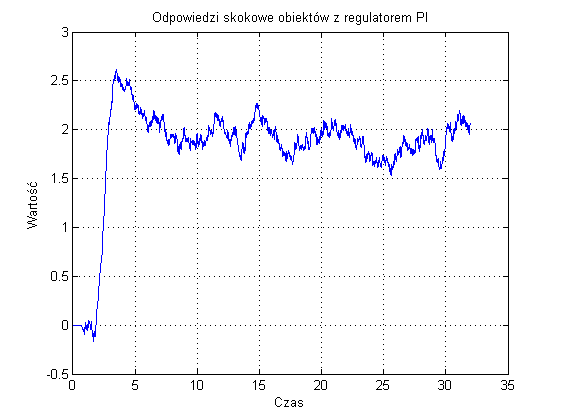
\includegraphics [width=4in]{skrypt_11.png}

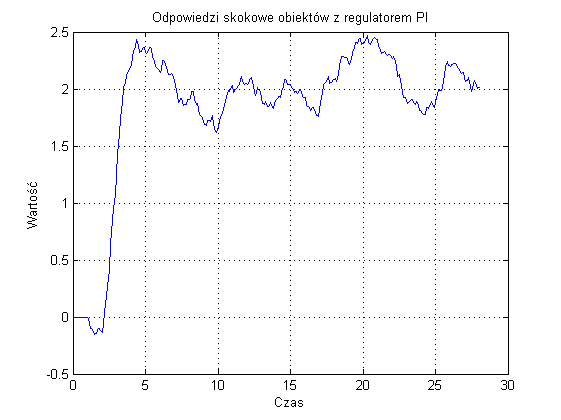
\includegraphics [width=4in]{skrypt_12.png}


\subsection*{P7}


        \color{lightgray} \begin{verbatim}Warning: The specified simulation stop time
(12.94) is not an integer multiple of the fixed
step size (0.0098999999999999991).  Changing the
stop time to (12.9393).  You can disable this
diagnostic by either specifying a stop time that
is an integer multiple of the fixed step size, or
setting 'Automatic solver parameter selection'
diagnostic to 'none' in the Diagnostics tab of
the Configuration Parameters dialog 
Warning: To use the default
trust-region-reflective algorithm you must supply
the gradient in the objective function and set
the GradObj option to 'on'. FMINCON will use the
active-set algorithm instead. For information on
applicable algorithms, see Choosing the Algorithm
in the documentation. 
Warning: Your current settings will run a
different algorithm (interior-point) in a future
release. 
Warning: The specified simulation stop time
(12.94) is not an integer multiple of the fixed
step size (0.0098999999999999991).  Changing the
stop time to (12.9393).  You can disable this
diagnostic by either specifying a stop time that
is an integer multiple of the fixed step size, or
setting 'Automatic solver parameter selection'
diagnostic to 'none' in the Diagnostics tab of
the Configuration Parameters dialog 
Warning: The specified simulation stop time
(12.94) is not an integer multiple of the fixed
step size (0.0098999999999999991).  Changing the
stop time to (12.9393).  You can disable this
diagnostic by either specifying a stop time that
is an integer multiple of the fixed step size, or
setting 'Automatic solver parameter selection'
diagnostic to 'none' in the Diagnostics tab of
the Configuration Parameters dialog 
Warning: The specified simulation stop time
(12.94) is not an integer multiple of the fixed
step size (0.0098999999999999991).  Changing the
stop time to (12.9393).  You can disable this
diagnostic by either specifying a stop time that
is an integer multiple of the fixed step size, or
setting 'Automatic solver parameter selection'
diagnostic to 'none' in the Diagnostics tab of
the Configuration Parameters dialog 
Warning: The specified simulation stop time
(12.94) is not an integer multiple of the fixed
step size (0.0098999999999999991).  Changing the
stop time to (12.9393).  You can disable this
diagnostic by either specifying a stop time that
is an integer multiple of the fixed step size, or
setting 'Automatic solver parameter selection'
diagnostic to 'none' in the Diagnostics tab of
the Configuration Parameters dialog 
Warning: The specified simulation stop time
(12.94) is not an integer multiple of the fixed
step size (0.0098999999999999991).  Changing the
stop time to (12.9393).  You can disable this
diagnostic by either specifying a stop time that
is an integer multiple of the fixed step size, or
setting 'Automatic solver parameter selection'
diagnostic to 'none' in the Diagnostics tab of
the Configuration Parameters dialog 
Warning: The specified simulation stop time
(12.94) is not an integer multiple of the fixed
step size (0.0098999999999999991).  Changing the
stop time to (12.9393).  You can disable this
diagnostic by either specifying a stop time that
is an integer multiple of the fixed step size, or
setting 'Automatic solver parameter selection'
diagnostic to 'none' in the Diagnostics tab of
the Configuration Parameters dialog 
Warning: The specified simulation stop time
(12.94) is not an integer multiple of the fixed
step size (0.0098999999999999991).  Changing the
stop time to (12.9393).  You can disable this
diagnostic by either specifying a stop time that
is an integer multiple of the fixed step size, or
setting 'Automatic solver parameter selection'
diagnostic to 'none' in the Diagnostics tab of
the Configuration Parameters dialog 
Warning: The specified simulation stop time
(12.94) is not an integer multiple of the fixed
step size (0.0098999999999999991).  Changing the
stop time to (12.9393).  You can disable this
diagnostic by either specifying a stop time that
is an integer multiple of the fixed step size, or
setting 'Automatic solver parameter selection'
diagnostic to 'none' in the Diagnostics tab of
the Configuration Parameters dialog 
Warning: The specified simulation stop time
(12.94) is not an integer multiple of the fixed
step size (0.0098999999999999991).  Changing the
stop time to (12.9393).  You can disable this
diagnostic by either specifying a stop time that
is an integer multiple of the fixed step size, or
setting 'Automatic solver parameter selection'
diagnostic to 'none' in the Diagnostics tab of
the Configuration Parameters dialog 
Warning: The specified simulation stop time
(12.94) is not an integer multiple of the fixed
step size (0.0098999999999999991).  Changing the
stop time to (12.9393).  You can disable this
diagnostic by either specifying a stop time that
is an integer multiple of the fixed step size, or
setting 'Automatic solver parameter selection'
diagnostic to 'none' in the Diagnostics tab of
the Configuration Parameters dialog 
Warning: The specified simulation stop time
(12.94) is not an integer multiple of the fixed
step size (0.0098999999999999991).  Changing the
stop time to (12.9393).  You can disable this
diagnostic by either specifying a stop time that
is an integer multiple of the fixed step size, or
setting 'Automatic solver parameter selection'
diagnostic to 'none' in the Diagnostics tab of
the Configuration Parameters dialog 
Warning: The specified simulation stop time
(12.94) is not an integer multiple of the fixed
step size (0.0098999999999999991).  Changing the
stop time to (12.9393).  You can disable this
diagnostic by either specifying a stop time that
is an integer multiple of the fixed step size, or
setting 'Automatic solver parameter selection'
diagnostic to 'none' in the Diagnostics tab of
the Configuration Parameters dialog 
Warning: The specified simulation stop time
(12.94) is not an integer multiple of the fixed
step size (0.0098999999999999991).  Changing the
stop time to (12.9393).  You can disable this
diagnostic by either specifying a stop time that
is an integer multiple of the fixed step size, or
setting 'Automatic solver parameter selection'
diagnostic to 'none' in the Diagnostics tab of
the Configuration Parameters dialog 
Warning: The specified simulation stop time
(12.94) is not an integer multiple of the fixed
step size (0.0098999999999999991).  Changing the
stop time to (12.9393).  You can disable this
diagnostic by either specifying a stop time that
is an integer multiple of the fixed step size, or
setting 'Automatic solver parameter selection'
diagnostic to 'none' in the Diagnostics tab of
the Configuration Parameters dialog 
Warning: The specified simulation stop time
(12.94) is not an integer multiple of the fixed
step size (0.0098999999999999991).  Changing the
stop time to (12.9393).  You can disable this
diagnostic by either specifying a stop time that
is an integer multiple of the fixed step size, or
setting 'Automatic solver parameter selection'
diagnostic to 'none' in the Diagnostics tab of
the Configuration Parameters dialog 
Warning: The specified simulation stop time
(12.94) is not an integer multiple of the fixed
step size (0.0098999999999999991).  Changing the
stop time to (12.9393).  You can disable this
diagnostic by either specifying a stop time that
is an integer multiple of the fixed step size, or
setting 'Automatic solver parameter selection'
diagnostic to 'none' in the Diagnostics tab of
the Configuration Parameters dialog 
Warning: The specified simulation stop time
(12.94) is not an integer multiple of the fixed
step size (0.0098999999999999991).  Changing the
stop time to (12.9393).  You can disable this
diagnostic by either specifying a stop time that
is an integer multiple of the fixed step size, or
setting 'Automatic solver parameter selection'
diagnostic to 'none' in the Diagnostics tab of
the Configuration Parameters dialog 
Warning: The specified simulation stop time
(12.94) is not an integer multiple of the fixed
step size (0.0098999999999999991).  Changing the
stop time to (12.9393).  You can disable this
diagnostic by either specifying a stop time that
is an integer multiple of the fixed step size, or
setting 'Automatic solver parameter selection'
diagnostic to 'none' in the Diagnostics tab of
the Configuration Parameters dialog 
Warning: The specified simulation stop time
(12.94) is not an integer multiple of the fixed
step size (0.0098999999999999991).  Changing the
stop time to (12.9393).  You can disable this
diagnostic by either specifying a stop time that
is an integer multiple of the fixed step size, or
setting 'Automatic solver parameter selection'
diagnostic to 'none' in the Diagnostics tab of
the Configuration Parameters dialog 
Warning: The specified simulation stop time
(12.94) is not an integer multiple of the fixed
step size (0.0098999999999999991).  Changing the
stop time to (12.9393).  You can disable this
diagnostic by either specifying a stop time that
is an integer multiple of the fixed step size, or
setting 'Automatic solver parameter selection'
diagnostic to 'none' in the Diagnostics tab of
the Configuration Parameters dialog 
Warning: The specified simulation stop time
(12.94) is not an integer multiple of the fixed
step size (0.0098999999999999991).  Changing the
stop time to (12.9393).  You can disable this
diagnostic by either specifying a stop time that
is an integer multiple of the fixed step size, or
setting 'Automatic solver parameter selection'
diagnostic to 'none' in the Diagnostics tab of
the Configuration Parameters dialog 
Warning: The specified simulation stop time
(12.94) is not an integer multiple of the fixed
step size (0.0098999999999999991).  Changing the
stop time to (12.9393).  You can disable this
diagnostic by either specifying a stop time that
is an integer multiple of the fixed step size, or
setting 'Automatic solver parameter selection'
diagnostic to 'none' in the Diagnostics tab of
the Configuration Parameters dialog 
Warning: The specified simulation stop time
(12.94) is not an integer multiple of the fixed
step size (0.0098999999999999991).  Changing the
stop time to (12.9393).  You can disable this
diagnostic by either specifying a stop time that
is an integer multiple of the fixed step size, or
setting 'Automatic solver parameter selection'
diagnostic to 'none' in the Diagnostics tab of
the Configuration Parameters dialog 
Warning: The specified simulation stop time
(12.94) is not an integer multiple of the fixed
step size (0.0098999999999999991).  Changing the
stop time to (12.9393).  You can disable this
diagnostic by either specifying a stop time that
is an integer multiple of the fixed step size, or
setting 'Automatic solver parameter selection'
diagnostic to 'none' in the Diagnostics tab of
the Configuration Parameters dialog 
Warning: The specified simulation stop time
(12.94) is not an integer multiple of the fixed
step size (0.0098999999999999991).  Changing the
stop time to (12.9393).  You can disable this
diagnostic by either specifying a stop time that
is an integer multiple of the fixed step size, or
setting 'Automatic solver parameter selection'
diagnostic to 'none' in the Diagnostics tab of
the Configuration Parameters dialog 
Warning: The specified simulation stop time
(12.94) is not an integer multiple of the fixed
step size (0.0098999999999999991).  Changing the
stop time to (12.9393).  You can disable this
diagnostic by either specifying a stop time that
is an integer multiple of the fixed step size, or
setting 'Automatic solver parameter selection'
diagnostic to 'none' in the Diagnostics tab of
the Configuration Parameters dialog 
Warning: The specified simulation stop time
(12.94) is not an integer multiple of the fixed
step size (0.0098999999999999991).  Changing the
stop time to (12.9393).  You can disable this
diagnostic by either specifying a stop time that
is an integer multiple of the fixed step size, or
setting 'Automatic solver parameter selection'
diagnostic to 'none' in the Diagnostics tab of
the Configuration Parameters dialog 
Warning: The specified simulation stop time
(12.94) is not an integer multiple of the fixed
step size (0.0098999999999999991).  Changing the
stop time to (12.9393).  You can disable this
diagnostic by either specifying a stop time that
is an integer multiple of the fixed step size, or
setting 'Automatic solver parameter selection'
diagnostic to 'none' in the Diagnostics tab of
the Configuration Parameters dialog 
Warning: The specified simulation stop time
(12.94) is not an integer multiple of the fixed
step size (0.0098999999999999991).  Changing the
stop time to (12.9393).  You can disable this
diagnostic by either specifying a stop time that
is an integer multiple of the fixed step size, or
setting 'Automatic solver parameter selection'
diagnostic to 'none' in the Diagnostics tab of
the Configuration Parameters dialog 
Warning: The specified simulation stop time
(12.94) is not an integer multiple of the fixed
step size (0.0098999999999999991).  Changing the
stop time to (12.9393).  You can disable this
diagnostic by either specifying a stop time that
is an integer multiple of the fixed step size, or
setting 'Automatic solver parameter selection'
diagnostic to 'none' in the Diagnostics tab of
the Configuration Parameters dialog 
Warning: The specified simulation stop time
(12.94) is not an integer multiple of the fixed
step size (0.0098999999999999991).  Changing the
stop time to (12.9393).  You can disable this
diagnostic by either specifying a stop time that
is an integer multiple of the fixed step size, or
setting 'Automatic solver parameter selection'
diagnostic to 'none' in the Diagnostics tab of
the Configuration Parameters dialog 
Warning: The specified simulation stop time
(12.94) is not an integer multiple of the fixed
step size (0.0098999999999999991).  Changing the
stop time to (12.9393).  You can disable this
diagnostic by either specifying a stop time that
is an integer multiple of the fixed step size, or
setting 'Automatic solver parameter selection'
diagnostic to 'none' in the Diagnostics tab of
the Configuration Parameters dialog 
Warning: The specified simulation stop time
(12.94) is not an integer multiple of the fixed
step size (0.0098999999999999991).  Changing the
stop time to (12.9393).  You can disable this
diagnostic by either specifying a stop time that
is an integer multiple of the fixed step size, or
setting 'Automatic solver parameter selection'
diagnostic to 'none' in the Diagnostics tab of
the Configuration Parameters dialog 
Warning: The specified simulation stop time
(12.94) is not an integer multiple of the fixed
step size (0.0098999999999999991).  Changing the
stop time to (12.9393).  You can disable this
diagnostic by either specifying a stop time that
is an integer multiple of the fixed step size, or
setting 'Automatic solver parameter selection'
diagnostic to 'none' in the Diagnostics tab of
the Configuration Parameters dialog 
Warning: The specified simulation stop time
(12.94) is not an integer multiple of the fixed
step size (0.0098999999999999991).  Changing the
stop time to (12.9393).  You can disable this
diagnostic by either specifying a stop time that
is an integer multiple of the fixed step size, or
setting 'Automatic solver parameter selection'
diagnostic to 'none' in the Diagnostics tab of
the Configuration Parameters dialog 
Warning: The specified simulation stop time
(12.94) is not an integer multiple of the fixed
step size (0.0098999999999999991).  Changing the
stop time to (12.9393).  You can disable this
diagnostic by either specifying a stop time that
is an integer multiple of the fixed step size, or
setting 'Automatic solver parameter selection'
diagnostic to 'none' in the Diagnostics tab of
the Configuration Parameters dialog 
Warning: The specified simulation stop time
(12.94) is not an integer multiple of the fixed
step size (0.0098999999999999991).  Changing the
stop time to (12.9393).  You can disable this
diagnostic by either specifying a stop time that
is an integer multiple of the fixed step size, or
setting 'Automatic solver parameter selection'
diagnostic to 'none' in the Diagnostics tab of
the Configuration Parameters dialog 
Warning: The specified simulation stop time
(12.94) is not an integer multiple of the fixed
step size (0.0098999999999999991).  Changing the
stop time to (12.9393).  You can disable this
diagnostic by either specifying a stop time that
is an integer multiple of the fixed step size, or
setting 'Automatic solver parameter selection'
diagnostic to 'none' in the Diagnostics tab of
the Configuration Parameters dialog 
Warning: The specified simulation stop time
(12.94) is not an integer multiple of the fixed
step size (0.0098999999999999991).  Changing the
stop time to (12.9393).  You can disable this
diagnostic by either specifying a stop time that
is an integer multiple of the fixed step size, or
setting 'Automatic solver parameter selection'
diagnostic to 'none' in the Diagnostics tab of
the Configuration Parameters dialog 
Warning: The specified simulation stop time
(12.94) is not an integer multiple of the fixed
step size (0.0098999999999999991).  Changing the
stop time to (12.9393).  You can disable this
diagnostic by either specifying a stop time that
is an integer multiple of the fixed step size, or
setting 'Automatic solver parameter selection'
diagnostic to 'none' in the Diagnostics tab of
the Configuration Parameters dialog 
Warning: The specified simulation stop time
(12.94) is not an integer multiple of the fixed
step size (0.0098999999999999991).  Changing the
stop time to (12.9393).  You can disable this
diagnostic by either specifying a stop time that
is an integer multiple of the fixed step size, or
setting 'Automatic solver parameter selection'
diagnostic to 'none' in the Diagnostics tab of
the Configuration Parameters dialog 
Warning: The specified simulation stop time
(12.94) is not an integer multiple of the fixed
step size (0.0098999999999999991).  Changing the
stop time to (12.9393).  You can disable this
diagnostic by either specifying a stop time that
is an integer multiple of the fixed step size, or
setting 'Automatic solver parameter selection'
diagnostic to 'none' in the Diagnostics tab of
the Configuration Parameters dialog 
Warning: The specified simulation stop time
(12.94) is not an integer multiple of the fixed
step size (0.0098999999999999991).  Changing the
stop time to (12.9393).  You can disable this
diagnostic by either specifying a stop time that
is an integer multiple of the fixed step size, or
setting 'Automatic solver parameter selection'
diagnostic to 'none' in the Diagnostics tab of
the Configuration Parameters dialog 
Warning: The specified simulation stop time
(12.94) is not an integer multiple of the fixed
step size (0.0098999999999999991).  Changing the
stop time to (12.9393).  You can disable this
diagnostic by either specifying a stop time that
is an integer multiple of the fixed step size, or
setting 'Automatic solver parameter selection'
diagnostic to 'none' in the Diagnostics tab of
the Configuration Parameters dialog 
Warning: The specified simulation stop time
(12.94) is not an integer multiple of the fixed
step size (0.0098999999999999991).  Changing the
stop time to (12.9393).  You can disable this
diagnostic by either specifying a stop time that
is an integer multiple of the fixed step size, or
setting 'Automatic solver parameter selection'
diagnostic to 'none' in the Diagnostics tab of
the Configuration Parameters dialog 
Warning: The specified simulation stop time
(12.94) is not an integer multiple of the fixed
step size (0.0098999999999999991).  Changing the
stop time to (12.9393).  You can disable this
diagnostic by either specifying a stop time that
is an integer multiple of the fixed step size, or
setting 'Automatic solver parameter selection'
diagnostic to 'none' in the Diagnostics tab of
the Configuration Parameters dialog 
Warning: The specified simulation stop time
(12.94) is not an integer multiple of the fixed
step size (0.0098999999999999991).  Changing the
stop time to (12.9393).  You can disable this
diagnostic by either specifying a stop time that
is an integer multiple of the fixed step size, or
setting 'Automatic solver parameter selection'
diagnostic to 'none' in the Diagnostics tab of
the Configuration Parameters dialog 
Warning: The specified simulation stop time
(12.94) is not an integer multiple of the fixed
step size (0.0098999999999999991).  Changing the
stop time to (12.9393).  You can disable this
diagnostic by either specifying a stop time that
is an integer multiple of the fixed step size, or
setting 'Automatic solver parameter selection'
diagnostic to 'none' in the Diagnostics tab of
the Configuration Parameters dialog 
Warning: The specified simulation stop time
(12.94) is not an integer multiple of the fixed
step size (0.0098999999999999991).  Changing the
stop time to (12.9393).  You can disable this
diagnostic by either specifying a stop time that
is an integer multiple of the fixed step size, or
setting 'Automatic solver parameter selection'
diagnostic to 'none' in the Diagnostics tab of
the Configuration Parameters dialog 

Local minimum possible. Constraints satisfied.

fmincon stopped because the predicted change in the objective function
is less than the default value of the function tolerance and constraints 
are satisfied to within the default value of the constraint tolerance.



No active inequalities.
Warning: The specified simulation stop time
(12.94) is not an integer multiple of the fixed
step size (0.0098999999999999991).  Changing the
stop time to (12.9393).  You can disable this
diagnostic by either specifying a stop time that
is an integer multiple of the fixed step size, or
setting 'Automatic solver parameter selection'
diagnostic to 'none' in the Diagnostics tab of
the Configuration Parameters dialog 
Warning: The specified simulation stop time
(34.94) is not an integer multiple of the fixed
step size (0.0098999999999999991).  Changing the
stop time to (34.937099999999994).  You can
disable this diagnostic by either specifying a
stop time that is an integer multiple of the
fixed step size, or setting 'Automatic solver
parameter selection' diagnostic to 'none' in the
Diagnostics tab of the Configuration Parameters
dialog 
Warning: To use the default
trust-region-reflective algorithm you must supply
the gradient in the objective function and set
the GradObj option to 'on'. FMINCON will use the
active-set algorithm instead. For information on
applicable algorithms, see Choosing the Algorithm
in the documentation. 
Warning: Your current settings will run a
different algorithm (interior-point) in a future
release. 

Local minimum possible. Constraints satisfied.

fmincon stopped because the predicted change in the objective function
is less than the default value of the function tolerance and constraints 
are satisfied to within the default value of the constraint tolerance.



No active inequalities.
Warning: The specified simulation stop time
(75.94) is not an integer multiple of the fixed
step size (0.0098999999999999991).  Changing the
stop time to (75.932999999999993).  You can
disable this diagnostic by either specifying a
stop time that is an integer multiple of the
fixed step size, or setting 'Automatic solver
parameter selection' diagnostic to 'none' in the
Diagnostics tab of the Configuration Parameters
dialog 
Warning: To use the default
trust-region-reflective algorithm you must supply
the gradient in the objective function and set
the GradObj option to 'on'. FMINCON will use the
active-set algorithm instead. For information on
applicable algorithms, see Choosing the Algorithm
in the documentation. 
Warning: Your current settings will run a
different algorithm (interior-point) in a future
release. 
Warning: The specified simulation stop time
(75.94) is not an integer multiple of the fixed
step size (0.0098999999999999991).  Changing the
stop time to (75.932999999999993).  You can
disable this diagnostic by either specifying a
stop time that is an integer multiple of the
fixed step size, or setting 'Automatic solver
parameter selection' diagnostic to 'none' in the
Diagnostics tab of the Configuration Parameters
dialog 
Warning: The specified simulation stop time
(75.94) is not an integer multiple of the fixed
step size (0.0098999999999999991).  Changing the
stop time to (75.932999999999993).  You can
disable this diagnostic by either specifying a
stop time that is an integer multiple of the
fixed step size, or setting 'Automatic solver
parameter selection' diagnostic to 'none' in the
Diagnostics tab of the Configuration Parameters
dialog 
Warning: The specified simulation stop time
(75.94) is not an integer multiple of the fixed
step size (0.0098999999999999991).  Changing the
stop time to (75.932999999999993).  You can
disable this diagnostic by either specifying a
stop time that is an integer multiple of the
fixed step size, or setting 'Automatic solver
parameter selection' diagnostic to 'none' in the
Diagnostics tab of the Configuration Parameters
dialog 
Warning: The specified simulation stop time
(75.94) is not an integer multiple of the fixed
step size (0.0098999999999999991).  Changing the
stop time to (75.932999999999993).  You can
disable this diagnostic by either specifying a
stop time that is an integer multiple of the
fixed step size, or setting 'Automatic solver
parameter selection' diagnostic to 'none' in the
Diagnostics tab of the Configuration Parameters
dialog 
Warning: The specified simulation stop time
(75.94) is not an integer multiple of the fixed
step size (0.0098999999999999991).  Changing the
stop time to (75.932999999999993).  You can
disable this diagnostic by either specifying a
stop time that is an integer multiple of the
fixed step size, or setting 'Automatic solver
parameter selection' diagnostic to 'none' in the
Diagnostics tab of the Configuration Parameters
dialog 
Warning: The specified simulation stop time
(75.94) is not an integer multiple of the fixed
step size (0.0098999999999999991).  Changing the
stop time to (75.932999999999993).  You can
disable this diagnostic by either specifying a
stop time that is an integer multiple of the
fixed step size, or setting 'Automatic solver
parameter selection' diagnostic to 'none' in the
Diagnostics tab of the Configuration Parameters
dialog 
Warning: The specified simulation stop time
(75.94) is not an integer multiple of the fixed
step size (0.0098999999999999991).  Changing the
stop time to (75.932999999999993).  You can
disable this diagnostic by either specifying a
stop time that is an integer multiple of the
fixed step size, or setting 'Automatic solver
parameter selection' diagnostic to 'none' in the
Diagnostics tab of the Configuration Parameters
dialog 
Warning: The specified simulation stop time
(75.94) is not an integer multiple of the fixed
step size (0.0098999999999999991).  Changing the
stop time to (75.932999999999993).  You can
disable this diagnostic by either specifying a
stop time that is an integer multiple of the
fixed step size, or setting 'Automatic solver
parameter selection' diagnostic to 'none' in the
Diagnostics tab of the Configuration Parameters
dialog 
Warning: The specified simulation stop time
(75.94) is not an integer multiple of the fixed
step size (0.0098999999999999991).  Changing the
stop time to (75.932999999999993).  You can
disable this diagnostic by either specifying a
stop time that is an integer multiple of the
fixed step size, or setting 'Automatic solver
parameter selection' diagnostic to 'none' in the
Diagnostics tab of the Configuration Parameters
dialog 
Warning: The specified simulation stop time
(75.94) is not an integer multiple of the fixed
step size (0.0098999999999999991).  Changing the
stop time to (75.932999999999993).  You can
disable this diagnostic by either specifying a
stop time that is an integer multiple of the
fixed step size, or setting 'Automatic solver
parameter selection' diagnostic to 'none' in the
Diagnostics tab of the Configuration Parameters
dialog 
Warning: The specified simulation stop time
(75.94) is not an integer multiple of the fixed
step size (0.0098999999999999991).  Changing the
stop time to (75.932999999999993).  You can
disable this diagnostic by either specifying a
stop time that is an integer multiple of the
fixed step size, or setting 'Automatic solver
parameter selection' diagnostic to 'none' in the
Diagnostics tab of the Configuration Parameters
dialog 
Warning: The specified simulation stop time
(75.94) is not an integer multiple of the fixed
step size (0.0098999999999999991).  Changing the
stop time to (75.932999999999993).  You can
disable this diagnostic by either specifying a
stop time that is an integer multiple of the
fixed step size, or setting 'Automatic solver
parameter selection' diagnostic to 'none' in the
Diagnostics tab of the Configuration Parameters
dialog 
Warning: The specified simulation stop time
(75.94) is not an integer multiple of the fixed
step size (0.0098999999999999991).  Changing the
stop time to (75.932999999999993).  You can
disable this diagnostic by either specifying a
stop time that is an integer multiple of the
fixed step size, or setting 'Automatic solver
parameter selection' diagnostic to 'none' in the
Diagnostics tab of the Configuration Parameters
dialog 
Warning: The specified simulation stop time
(75.94) is not an integer multiple of the fixed
step size (0.0098999999999999991).  Changing the
stop time to (75.932999999999993).  You can
disable this diagnostic by either specifying a
stop time that is an integer multiple of the
fixed step size, or setting 'Automatic solver
parameter selection' diagnostic to 'none' in the
Diagnostics tab of the Configuration Parameters
dialog 
Warning: The specified simulation stop time
(75.94) is not an integer multiple of the fixed
step size (0.0098999999999999991).  Changing the
stop time to (75.932999999999993).  You can
disable this diagnostic by either specifying a
stop time that is an integer multiple of the
fixed step size, or setting 'Automatic solver
parameter selection' diagnostic to 'none' in the
Diagnostics tab of the Configuration Parameters
dialog 
Warning: The specified simulation stop time
(75.94) is not an integer multiple of the fixed
step size (0.0098999999999999991).  Changing the
stop time to (75.932999999999993).  You can
disable this diagnostic by either specifying a
stop time that is an integer multiple of the
fixed step size, or setting 'Automatic solver
parameter selection' diagnostic to 'none' in the
Diagnostics tab of the Configuration Parameters
dialog 
Warning: The specified simulation stop time
(75.94) is not an integer multiple of the fixed
step size (0.0098999999999999991).  Changing the
stop time to (75.932999999999993).  You can
disable this diagnostic by either specifying a
stop time that is an integer multiple of the
fixed step size, or setting 'Automatic solver
parameter selection' diagnostic to 'none' in the
Diagnostics tab of the Configuration Parameters
dialog 
Warning: The specified simulation stop time
(75.94) is not an integer multiple of the fixed
step size (0.0098999999999999991).  Changing the
stop time to (75.932999999999993).  You can
disable this diagnostic by either specifying a
stop time that is an integer multiple of the
fixed step size, or setting 'Automatic solver
parameter selection' diagnostic to 'none' in the
Diagnostics tab of the Configuration Parameters
dialog 
Warning: The specified simulation stop time
(75.94) is not an integer multiple of the fixed
step size (0.0098999999999999991).  Changing the
stop time to (75.932999999999993).  You can
disable this diagnostic by either specifying a
stop time that is an integer multiple of the
fixed step size, or setting 'Automatic solver
parameter selection' diagnostic to 'none' in the
Diagnostics tab of the Configuration Parameters
dialog 
Warning: The specified simulation stop time
(75.94) is not an integer multiple of the fixed
step size (0.0098999999999999991).  Changing the
stop time to (75.932999999999993).  You can
disable this diagnostic by either specifying a
stop time that is an integer multiple of the
fixed step size, or setting 'Automatic solver
parameter selection' diagnostic to 'none' in the
Diagnostics tab of the Configuration Parameters
dialog 
Warning: The specified simulation stop time
(75.94) is not an integer multiple of the fixed
step size (0.0098999999999999991).  Changing the
stop time to (75.932999999999993).  You can
disable this diagnostic by either specifying a
stop time that is an integer multiple of the
fixed step size, or setting 'Automatic solver
parameter selection' diagnostic to 'none' in the
Diagnostics tab of the Configuration Parameters
dialog 
Warning: The specified simulation stop time
(75.94) is not an integer multiple of the fixed
step size (0.0098999999999999991).  Changing the
stop time to (75.932999999999993).  You can
disable this diagnostic by either specifying a
stop time that is an integer multiple of the
fixed step size, or setting 'Automatic solver
parameter selection' diagnostic to 'none' in the
Diagnostics tab of the Configuration Parameters
dialog 
Warning: The specified simulation stop time
(75.94) is not an integer multiple of the fixed
step size (0.0098999999999999991).  Changing the
stop time to (75.932999999999993).  You can
disable this diagnostic by either specifying a
stop time that is an integer multiple of the
fixed step size, or setting 'Automatic solver
parameter selection' diagnostic to 'none' in the
Diagnostics tab of the Configuration Parameters
dialog 
Warning: The specified simulation stop time
(75.94) is not an integer multiple of the fixed
step size (0.0098999999999999991).  Changing the
stop time to (75.932999999999993).  You can
disable this diagnostic by either specifying a
stop time that is an integer multiple of the
fixed step size, or setting 'Automatic solver
parameter selection' diagnostic to 'none' in the
Diagnostics tab of the Configuration Parameters
dialog 
Warning: The specified simulation stop time
(75.94) is not an integer multiple of the fixed
step size (0.0098999999999999991).  Changing the
stop time to (75.932999999999993).  You can
disable this diagnostic by either specifying a
stop time that is an integer multiple of the
fixed step size, or setting 'Automatic solver
parameter selection' diagnostic to 'none' in the
Diagnostics tab of the Configuration Parameters
dialog 
Warning: The specified simulation stop time
(75.94) is not an integer multiple of the fixed
step size (0.0098999999999999991).  Changing the
stop time to (75.932999999999993).  You can
disable this diagnostic by either specifying a
stop time that is an integer multiple of the
fixed step size, or setting 'Automatic solver
parameter selection' diagnostic to 'none' in the
Diagnostics tab of the Configuration Parameters
dialog 
Warning: The specified simulation stop time
(75.94) is not an integer multiple of the fixed
step size (0.0098999999999999991).  Changing the
stop time to (75.932999999999993).  You can
disable this diagnostic by either specifying a
stop time that is an integer multiple of the
fixed step size, or setting 'Automatic solver
parameter selection' diagnostic to 'none' in the
Diagnostics tab of the Configuration Parameters
dialog 
Warning: The specified simulation stop time
(75.94) is not an integer multiple of the fixed
step size (0.0098999999999999991).  Changing the
stop time to (75.932999999999993).  You can
disable this diagnostic by either specifying a
stop time that is an integer multiple of the
fixed step size, or setting 'Automatic solver
parameter selection' diagnostic to 'none' in the
Diagnostics tab of the Configuration Parameters
dialog 
Warning: The specified simulation stop time
(75.94) is not an integer multiple of the fixed
step size (0.0098999999999999991).  Changing the
stop time to (75.932999999999993).  You can
disable this diagnostic by either specifying a
stop time that is an integer multiple of the
fixed step size, or setting 'Automatic solver
parameter selection' diagnostic to 'none' in the
Diagnostics tab of the Configuration Parameters
dialog 
Warning: The specified simulation stop time
(75.94) is not an integer multiple of the fixed
step size (0.0098999999999999991).  Changing the
stop time to (75.932999999999993).  You can
disable this diagnostic by either specifying a
stop time that is an integer multiple of the
fixed step size, or setting 'Automatic solver
parameter selection' diagnostic to 'none' in the
Diagnostics tab of the Configuration Parameters
dialog 
Warning: The specified simulation stop time
(75.94) is not an integer multiple of the fixed
step size (0.0098999999999999991).  Changing the
stop time to (75.932999999999993).  You can
disable this diagnostic by either specifying a
stop time that is an integer multiple of the
fixed step size, or setting 'Automatic solver
parameter selection' diagnostic to 'none' in the
Diagnostics tab of the Configuration Parameters
dialog 
Warning: The specified simulation stop time
(75.94) is not an integer multiple of the fixed
step size (0.0098999999999999991).  Changing the
stop time to (75.932999999999993).  You can
disable this diagnostic by either specifying a
stop time that is an integer multiple of the
fixed step size, or setting 'Automatic solver
parameter selection' diagnostic to 'none' in the
Diagnostics tab of the Configuration Parameters
dialog 
Warning: The specified simulation stop time
(75.94) is not an integer multiple of the fixed
step size (0.0098999999999999991).  Changing the
stop time to (75.932999999999993).  You can
disable this diagnostic by either specifying a
stop time that is an integer multiple of the
fixed step size, or setting 'Automatic solver
parameter selection' diagnostic to 'none' in the
Diagnostics tab of the Configuration Parameters
dialog 
Warning: The specified simulation stop time
(75.94) is not an integer multiple of the fixed
step size (0.0098999999999999991).  Changing the
stop time to (75.932999999999993).  You can
disable this diagnostic by either specifying a
stop time that is an integer multiple of the
fixed step size, or setting 'Automatic solver
parameter selection' diagnostic to 'none' in the
Diagnostics tab of the Configuration Parameters
dialog 
Warning: The specified simulation stop time
(75.94) is not an integer multiple of the fixed
step size (0.0098999999999999991).  Changing the
stop time to (75.932999999999993).  You can
disable this diagnostic by either specifying a
stop time that is an integer multiple of the
fixed step size, or setting 'Automatic solver
parameter selection' diagnostic to 'none' in the
Diagnostics tab of the Configuration Parameters
dialog 
Warning: The specified simulation stop time
(75.94) is not an integer multiple of the fixed
step size (0.0098999999999999991).  Changing the
stop time to (75.932999999999993).  You can
disable this diagnostic by either specifying a
stop time that is an integer multiple of the
fixed step size, or setting 'Automatic solver
parameter selection' diagnostic to 'none' in the
Diagnostics tab of the Configuration Parameters
dialog 
Warning: The specified simulation stop time
(75.94) is not an integer multiple of the fixed
step size (0.0098999999999999991).  Changing the
stop time to (75.932999999999993).  You can
disable this diagnostic by either specifying a
stop time that is an integer multiple of the
fixed step size, or setting 'Automatic solver
parameter selection' diagnostic to 'none' in the
Diagnostics tab of the Configuration Parameters
dialog 
Warning: The specified simulation stop time
(75.94) is not an integer multiple of the fixed
step size (0.0098999999999999991).  Changing the
stop time to (75.932999999999993).  You can
disable this diagnostic by either specifying a
stop time that is an integer multiple of the
fixed step size, or setting 'Automatic solver
parameter selection' diagnostic to 'none' in the
Diagnostics tab of the Configuration Parameters
dialog 
Warning: The specified simulation stop time
(75.94) is not an integer multiple of the fixed
step size (0.0098999999999999991).  Changing the
stop time to (75.932999999999993).  You can
disable this diagnostic by either specifying a
stop time that is an integer multiple of the
fixed step size, or setting 'Automatic solver
parameter selection' diagnostic to 'none' in the
Diagnostics tab of the Configuration Parameters
dialog 
Warning: The specified simulation stop time
(75.94) is not an integer multiple of the fixed
step size (0.0098999999999999991).  Changing the
stop time to (75.932999999999993).  You can
disable this diagnostic by either specifying a
stop time that is an integer multiple of the
fixed step size, or setting 'Automatic solver
parameter selection' diagnostic to 'none' in the
Diagnostics tab of the Configuration Parameters
dialog 
Warning: The specified simulation stop time
(75.94) is not an integer multiple of the fixed
step size (0.0098999999999999991).  Changing the
stop time to (75.932999999999993).  You can
disable this diagnostic by either specifying a
stop time that is an integer multiple of the
fixed step size, or setting 'Automatic solver
parameter selection' diagnostic to 'none' in the
Diagnostics tab of the Configuration Parameters
dialog 
Warning: The specified simulation stop time
(75.94) is not an integer multiple of the fixed
step size (0.0098999999999999991).  Changing the
stop time to (75.932999999999993).  You can
disable this diagnostic by either specifying a
stop time that is an integer multiple of the
fixed step size, or setting 'Automatic solver
parameter selection' diagnostic to 'none' in the
Diagnostics tab of the Configuration Parameters
dialog 
Warning: The specified simulation stop time
(75.94) is not an integer multiple of the fixed
step size (0.0098999999999999991).  Changing the
stop time to (75.932999999999993).  You can
disable this diagnostic by either specifying a
stop time that is an integer multiple of the
fixed step size, or setting 'Automatic solver
parameter selection' diagnostic to 'none' in the
Diagnostics tab of the Configuration Parameters
dialog 
Warning: The specified simulation stop time
(75.94) is not an integer multiple of the fixed
step size (0.0098999999999999991).  Changing the
stop time to (75.932999999999993).  You can
disable this diagnostic by either specifying a
stop time that is an integer multiple of the
fixed step size, or setting 'Automatic solver
parameter selection' diagnostic to 'none' in the
Diagnostics tab of the Configuration Parameters
dialog 
Warning: The specified simulation stop time
(75.94) is not an integer multiple of the fixed
step size (0.0098999999999999991).  Changing the
stop time to (75.932999999999993).  You can
disable this diagnostic by either specifying a
stop time that is an integer multiple of the
fixed step size, or setting 'Automatic solver
parameter selection' diagnostic to 'none' in the
Diagnostics tab of the Configuration Parameters
dialog 
Warning: The specified simulation stop time
(75.94) is not an integer multiple of the fixed
step size (0.0098999999999999991).  Changing the
stop time to (75.932999999999993).  You can
disable this diagnostic by either specifying a
stop time that is an integer multiple of the
fixed step size, or setting 'Automatic solver
parameter selection' diagnostic to 'none' in the
Diagnostics tab of the Configuration Parameters
dialog 
Warning: The specified simulation stop time
(75.94) is not an integer multiple of the fixed
step size (0.0098999999999999991).  Changing the
stop time to (75.932999999999993).  You can
disable this diagnostic by either specifying a
stop time that is an integer multiple of the
fixed step size, or setting 'Automatic solver
parameter selection' diagnostic to 'none' in the
Diagnostics tab of the Configuration Parameters
dialog 
Warning: The specified simulation stop time
(75.94) is not an integer multiple of the fixed
step size (0.0098999999999999991).  Changing the
stop time to (75.932999999999993).  You can
disable this diagnostic by either specifying a
stop time that is an integer multiple of the
fixed step size, or setting 'Automatic solver
parameter selection' diagnostic to 'none' in the
Diagnostics tab of the Configuration Parameters
dialog 
Warning: The specified simulation stop time
(75.94) is not an integer multiple of the fixed
step size (0.0098999999999999991).  Changing the
stop time to (75.932999999999993).  You can
disable this diagnostic by either specifying a
stop time that is an integer multiple of the
fixed step size, or setting 'Automatic solver
parameter selection' diagnostic to 'none' in the
Diagnostics tab of the Configuration Parameters
dialog 
Warning: The specified simulation stop time
(75.94) is not an integer multiple of the fixed
step size (0.0098999999999999991).  Changing the
stop time to (75.932999999999993).  You can
disable this diagnostic by either specifying a
stop time that is an integer multiple of the
fixed step size, or setting 'Automatic solver
parameter selection' diagnostic to 'none' in the
Diagnostics tab of the Configuration Parameters
dialog 
Warning: The specified simulation stop time
(75.94) is not an integer multiple of the fixed
step size (0.0098999999999999991).  Changing the
stop time to (75.932999999999993).  You can
disable this diagnostic by either specifying a
stop time that is an integer multiple of the
fixed step size, or setting 'Automatic solver
parameter selection' diagnostic to 'none' in the
Diagnostics tab of the Configuration Parameters
dialog 
Warning: The specified simulation stop time
(75.94) is not an integer multiple of the fixed
step size (0.0098999999999999991).  Changing the
stop time to (75.932999999999993).  You can
disable this diagnostic by either specifying a
stop time that is an integer multiple of the
fixed step size, or setting 'Automatic solver
parameter selection' diagnostic to 'none' in the
Diagnostics tab of the Configuration Parameters
dialog 
Warning: The specified simulation stop time
(75.94) is not an integer multiple of the fixed
step size (0.0098999999999999991).  Changing the
stop time to (75.932999999999993).  You can
disable this diagnostic by either specifying a
stop time that is an integer multiple of the
fixed step size, or setting 'Automatic solver
parameter selection' diagnostic to 'none' in the
Diagnostics tab of the Configuration Parameters
dialog 
Warning: The specified simulation stop time
(75.94) is not an integer multiple of the fixed
step size (0.0098999999999999991).  Changing the
stop time to (75.932999999999993).  You can
disable this diagnostic by either specifying a
stop time that is an integer multiple of the
fixed step size, or setting 'Automatic solver
parameter selection' diagnostic to 'none' in the
Diagnostics tab of the Configuration Parameters
dialog 
Warning: The specified simulation stop time
(75.94) is not an integer multiple of the fixed
step size (0.0098999999999999991).  Changing the
stop time to (75.932999999999993).  You can
disable this diagnostic by either specifying a
stop time that is an integer multiple of the
fixed step size, or setting 'Automatic solver
parameter selection' diagnostic to 'none' in the
Diagnostics tab of the Configuration Parameters
dialog 
Warning: The specified simulation stop time
(75.94) is not an integer multiple of the fixed
step size (0.0098999999999999991).  Changing the
stop time to (75.932999999999993).  You can
disable this diagnostic by either specifying a
stop time that is an integer multiple of the
fixed step size, or setting 'Automatic solver
parameter selection' diagnostic to 'none' in the
Diagnostics tab of the Configuration Parameters
dialog 
Warning: The specified simulation stop time
(75.94) is not an integer multiple of the fixed
step size (0.0098999999999999991).  Changing the
stop time to (75.932999999999993).  You can
disable this diagnostic by either specifying a
stop time that is an integer multiple of the
fixed step size, or setting 'Automatic solver
parameter selection' diagnostic to 'none' in the
Diagnostics tab of the Configuration Parameters
dialog 
Warning: The specified simulation stop time
(75.94) is not an integer multiple of the fixed
step size (0.0098999999999999991).  Changing the
stop time to (75.932999999999993).  You can
disable this diagnostic by either specifying a
stop time that is an integer multiple of the
fixed step size, or setting 'Automatic solver
parameter selection' diagnostic to 'none' in the
Diagnostics tab of the Configuration Parameters
dialog 
Warning: The specified simulation stop time
(75.94) is not an integer multiple of the fixed
step size (0.0098999999999999991).  Changing the
stop time to (75.932999999999993).  You can
disable this diagnostic by either specifying a
stop time that is an integer multiple of the
fixed step size, or setting 'Automatic solver
parameter selection' diagnostic to 'none' in the
Diagnostics tab of the Configuration Parameters
dialog 
Warning: The specified simulation stop time
(75.94) is not an integer multiple of the fixed
step size (0.0098999999999999991).  Changing the
stop time to (75.932999999999993).  You can
disable this diagnostic by either specifying a
stop time that is an integer multiple of the
fixed step size, or setting 'Automatic solver
parameter selection' diagnostic to 'none' in the
Diagnostics tab of the Configuration Parameters
dialog 
Warning: The specified simulation stop time
(75.94) is not an integer multiple of the fixed
step size (0.0098999999999999991).  Changing the
stop time to (75.932999999999993).  You can
disable this diagnostic by either specifying a
stop time that is an integer multiple of the
fixed step size, or setting 'Automatic solver
parameter selection' diagnostic to 'none' in the
Diagnostics tab of the Configuration Parameters
dialog 
Warning: The specified simulation stop time
(75.94) is not an integer multiple of the fixed
step size (0.0098999999999999991).  Changing the
stop time to (75.932999999999993).  You can
disable this diagnostic by either specifying a
stop time that is an integer multiple of the
fixed step size, or setting 'Automatic solver
parameter selection' diagnostic to 'none' in the
Diagnostics tab of the Configuration Parameters
dialog 
Warning: The specified simulation stop time
(75.94) is not an integer multiple of the fixed
step size (0.0098999999999999991).  Changing the
stop time to (75.932999999999993).  You can
disable this diagnostic by either specifying a
stop time that is an integer multiple of the
fixed step size, or setting 'Automatic solver
parameter selection' diagnostic to 'none' in the
Diagnostics tab of the Configuration Parameters
dialog 
Warning: The specified simulation stop time
(75.94) is not an integer multiple of the fixed
step size (0.0098999999999999991).  Changing the
stop time to (75.932999999999993).  You can
disable this diagnostic by either specifying a
stop time that is an integer multiple of the
fixed step size, or setting 'Automatic solver
parameter selection' diagnostic to 'none' in the
Diagnostics tab of the Configuration Parameters
dialog 
Warning: The specified simulation stop time
(75.94) is not an integer multiple of the fixed
step size (0.0098999999999999991).  Changing the
stop time to (75.932999999999993).  You can
disable this diagnostic by either specifying a
stop time that is an integer multiple of the
fixed step size, or setting 'Automatic solver
parameter selection' diagnostic to 'none' in the
Diagnostics tab of the Configuration Parameters
dialog 
Warning: The specified simulation stop time
(75.94) is not an integer multiple of the fixed
step size (0.0098999999999999991).  Changing the
stop time to (75.932999999999993).  You can
disable this diagnostic by either specifying a
stop time that is an integer multiple of the
fixed step size, or setting 'Automatic solver
parameter selection' diagnostic to 'none' in the
Diagnostics tab of the Configuration Parameters
dialog 
Warning: The specified simulation stop time
(75.94) is not an integer multiple of the fixed
step size (0.0098999999999999991).  Changing the
stop time to (75.932999999999993).  You can
disable this diagnostic by either specifying a
stop time that is an integer multiple of the
fixed step size, or setting 'Automatic solver
parameter selection' diagnostic to 'none' in the
Diagnostics tab of the Configuration Parameters
dialog 
Warning: The specified simulation stop time
(75.94) is not an integer multiple of the fixed
step size (0.0098999999999999991).  Changing the
stop time to (75.932999999999993).  You can
disable this diagnostic by either specifying a
stop time that is an integer multiple of the
fixed step size, or setting 'Automatic solver
parameter selection' diagnostic to 'none' in the
Diagnostics tab of the Configuration Parameters
dialog 
Warning: The specified simulation stop time
(75.94) is not an integer multiple of the fixed
step size (0.0098999999999999991).  Changing the
stop time to (75.932999999999993).  You can
disable this diagnostic by either specifying a
stop time that is an integer multiple of the
fixed step size, or setting 'Automatic solver
parameter selection' diagnostic to 'none' in the
Diagnostics tab of the Configuration Parameters
dialog 
Warning: The specified simulation stop time
(75.94) is not an integer multiple of the fixed
step size (0.0098999999999999991).  Changing the
stop time to (75.932999999999993).  You can
disable this diagnostic by either specifying a
stop time that is an integer multiple of the
fixed step size, or setting 'Automatic solver
parameter selection' diagnostic to 'none' in the
Diagnostics tab of the Configuration Parameters
dialog 
Warning: The specified simulation stop time
(75.94) is not an integer multiple of the fixed
step size (0.0098999999999999991).  Changing the
stop time to (75.932999999999993).  You can
disable this diagnostic by either specifying a
stop time that is an integer multiple of the
fixed step size, or setting 'Automatic solver
parameter selection' diagnostic to 'none' in the
Diagnostics tab of the Configuration Parameters
dialog 
Warning: The specified simulation stop time
(75.94) is not an integer multiple of the fixed
step size (0.0098999999999999991).  Changing the
stop time to (75.932999999999993).  You can
disable this diagnostic by either specifying a
stop time that is an integer multiple of the
fixed step size, or setting 'Automatic solver
parameter selection' diagnostic to 'none' in the
Diagnostics tab of the Configuration Parameters
dialog 
Warning: The specified simulation stop time
(75.94) is not an integer multiple of the fixed
step size (0.0098999999999999991).  Changing the
stop time to (75.932999999999993).  You can
disable this diagnostic by either specifying a
stop time that is an integer multiple of the
fixed step size, or setting 'Automatic solver
parameter selection' diagnostic to 'none' in the
Diagnostics tab of the Configuration Parameters
dialog 
Warning: The specified simulation stop time
(75.94) is not an integer multiple of the fixed
step size (0.0098999999999999991).  Changing the
stop time to (75.932999999999993).  You can
disable this diagnostic by either specifying a
stop time that is an integer multiple of the
fixed step size, or setting 'Automatic solver
parameter selection' diagnostic to 'none' in the
Diagnostics tab of the Configuration Parameters
dialog 
Warning: The specified simulation stop time
(75.94) is not an integer multiple of the fixed
step size (0.0098999999999999991).  Changing the
stop time to (75.932999999999993).  You can
disable this diagnostic by either specifying a
stop time that is an integer multiple of the
fixed step size, or setting 'Automatic solver
parameter selection' diagnostic to 'none' in the
Diagnostics tab of the Configuration Parameters
dialog 
Warning: The specified simulation stop time
(75.94) is not an integer multiple of the fixed
step size (0.0098999999999999991).  Changing the
stop time to (75.932999999999993).  You can
disable this diagnostic by either specifying a
stop time that is an integer multiple of the
fixed step size, or setting 'Automatic solver
parameter selection' diagnostic to 'none' in the
Diagnostics tab of the Configuration Parameters
dialog 
Warning: The specified simulation stop time
(75.94) is not an integer multiple of the fixed
step size (0.0098999999999999991).  Changing the
stop time to (75.932999999999993).  You can
disable this diagnostic by either specifying a
stop time that is an integer multiple of the
fixed step size, or setting 'Automatic solver
parameter selection' diagnostic to 'none' in the
Diagnostics tab of the Configuration Parameters
dialog 
Warning: The specified simulation stop time
(75.94) is not an integer multiple of the fixed
step size (0.0098999999999999991).  Changing the
stop time to (75.932999999999993).  You can
disable this diagnostic by either specifying a
stop time that is an integer multiple of the
fixed step size, or setting 'Automatic solver
parameter selection' diagnostic to 'none' in the
Diagnostics tab of the Configuration Parameters
dialog 
Warning: The specified simulation stop time
(75.94) is not an integer multiple of the fixed
step size (0.0098999999999999991).  Changing the
stop time to (75.932999999999993).  You can
disable this diagnostic by either specifying a
stop time that is an integer multiple of the
fixed step size, or setting 'Automatic solver
parameter selection' diagnostic to 'none' in the
Diagnostics tab of the Configuration Parameters
dialog 
Warning: The specified simulation stop time
(75.94) is not an integer multiple of the fixed
step size (0.0098999999999999991).  Changing the
stop time to (75.932999999999993).  You can
disable this diagnostic by either specifying a
stop time that is an integer multiple of the
fixed step size, or setting 'Automatic solver
parameter selection' diagnostic to 'none' in the
Diagnostics tab of the Configuration Parameters
dialog 
Warning: The specified simulation stop time
(75.94) is not an integer multiple of the fixed
step size (0.0098999999999999991).  Changing the
stop time to (75.932999999999993).  You can
disable this diagnostic by either specifying a
stop time that is an integer multiple of the
fixed step size, or setting 'Automatic solver
parameter selection' diagnostic to 'none' in the
Diagnostics tab of the Configuration Parameters
dialog 
Warning: The specified simulation stop time
(75.94) is not an integer multiple of the fixed
step size (0.0098999999999999991).  Changing the
stop time to (75.932999999999993).  You can
disable this diagnostic by either specifying a
stop time that is an integer multiple of the
fixed step size, or setting 'Automatic solver
parameter selection' diagnostic to 'none' in the
Diagnostics tab of the Configuration Parameters
dialog 
Warning: The specified simulation stop time
(75.94) is not an integer multiple of the fixed
step size (0.0098999999999999991).  Changing the
stop time to (75.932999999999993).  You can
disable this diagnostic by either specifying a
stop time that is an integer multiple of the
fixed step size, or setting 'Automatic solver
parameter selection' diagnostic to 'none' in the
Diagnostics tab of the Configuration Parameters
dialog 
Warning: The specified simulation stop time
(75.94) is not an integer multiple of the fixed
step size (0.0098999999999999991).  Changing the
stop time to (75.932999999999993).  You can
disable this diagnostic by either specifying a
stop time that is an integer multiple of the
fixed step size, or setting 'Automatic solver
parameter selection' diagnostic to 'none' in the
Diagnostics tab of the Configuration Parameters
dialog 
Warning: The specified simulation stop time
(75.94) is not an integer multiple of the fixed
step size (0.0098999999999999991).  Changing the
stop time to (75.932999999999993).  You can
disable this diagnostic by either specifying a
stop time that is an integer multiple of the
fixed step size, or setting 'Automatic solver
parameter selection' diagnostic to 'none' in the
Diagnostics tab of the Configuration Parameters
dialog 
Warning: The specified simulation stop time
(75.94) is not an integer multiple of the fixed
step size (0.0098999999999999991).  Changing the
stop time to (75.932999999999993).  You can
disable this diagnostic by either specifying a
stop time that is an integer multiple of the
fixed step size, or setting 'Automatic solver
parameter selection' diagnostic to 'none' in the
Diagnostics tab of the Configuration Parameters
dialog 
Warning: The specified simulation stop time
(75.94) is not an integer multiple of the fixed
step size (0.0098999999999999991).  Changing the
stop time to (75.932999999999993).  You can
disable this diagnostic by either specifying a
stop time that is an integer multiple of the
fixed step size, or setting 'Automatic solver
parameter selection' diagnostic to 'none' in the
Diagnostics tab of the Configuration Parameters
dialog 
Warning: The specified simulation stop time
(75.94) is not an integer multiple of the fixed
step size (0.0098999999999999991).  Changing the
stop time to (75.932999999999993).  You can
disable this diagnostic by either specifying a
stop time that is an integer multiple of the
fixed step size, or setting 'Automatic solver
parameter selection' diagnostic to 'none' in the
Diagnostics tab of the Configuration Parameters
dialog 
Warning: The specified simulation stop time
(75.94) is not an integer multiple of the fixed
step size (0.0098999999999999991).  Changing the
stop time to (75.932999999999993).  You can
disable this diagnostic by either specifying a
stop time that is an integer multiple of the
fixed step size, or setting 'Automatic solver
parameter selection' diagnostic to 'none' in the
Diagnostics tab of the Configuration Parameters
dialog 
Warning: The specified simulation stop time
(75.94) is not an integer multiple of the fixed
step size (0.0098999999999999991).  Changing the
stop time to (75.932999999999993).  You can
disable this diagnostic by either specifying a
stop time that is an integer multiple of the
fixed step size, or setting 'Automatic solver
parameter selection' diagnostic to 'none' in the
Diagnostics tab of the Configuration Parameters
dialog 
Warning: The specified simulation stop time
(75.94) is not an integer multiple of the fixed
step size (0.0098999999999999991).  Changing the
stop time to (75.932999999999993).  You can
disable this diagnostic by either specifying a
stop time that is an integer multiple of the
fixed step size, or setting 'Automatic solver
parameter selection' diagnostic to 'none' in the
Diagnostics tab of the Configuration Parameters
dialog 
Warning: The specified simulation stop time
(75.94) is not an integer multiple of the fixed
step size (0.0098999999999999991).  Changing the
stop time to (75.932999999999993).  You can
disable this diagnostic by either specifying a
stop time that is an integer multiple of the
fixed step size, or setting 'Automatic solver
parameter selection' diagnostic to 'none' in the
Diagnostics tab of the Configuration Parameters
dialog 
Warning: The specified simulation stop time
(75.94) is not an integer multiple of the fixed
step size (0.0098999999999999991).  Changing the
stop time to (75.932999999999993).  You can
disable this diagnostic by either specifying a
stop time that is an integer multiple of the
fixed step size, or setting 'Automatic solver
parameter selection' diagnostic to 'none' in the
Diagnostics tab of the Configuration Parameters
dialog 

Local minimum possible. Constraints satisfied.

fmincon stopped because the predicted change in the objective function
is less than the default value of the function tolerance and constraints 
are satisfied to within the default value of the constraint tolerance.



No active inequalities.
Warning: The specified simulation stop time
(75.94) is not an integer multiple of the fixed
step size (0.0098999999999999991).  Changing the
stop time to (75.932999999999993).  You can
disable this diagnostic by either specifying a
stop time that is an integer multiple of the
fixed step size, or setting 'Automatic solver
parameter selection' diagnostic to 'none' in the
Diagnostics tab of the Configuration Parameters
dialog 
Warning: The specified simulation stop time
(115.94) is not an integer multiple of the fixed
step size (0.0098999999999999991).  Changing the
stop time to (115.93889999999999).  You can
disable this diagnostic by either specifying a
stop time that is an integer multiple of the
fixed step size, or setting 'Automatic solver
parameter selection' diagnostic to 'none' in the
Diagnostics tab of the Configuration Parameters
dialog 
Warning: To use the default
trust-region-reflective algorithm you must supply
the gradient in the objective function and set
the GradObj option to 'on'. FMINCON will use the
active-set algorithm instead. For information on
applicable algorithms, see Choosing the Algorithm
in the documentation. 
Warning: Your current settings will run a
different algorithm (interior-point) in a future
release. 
Warning: The specified delay time for
'single_object/Transport Delay' is smaller than
the step size of the fixed-step solver. This may
cause simulation results to be inaccurate.
Consider decreasing the step size of the solver
to improve accuracy 
Warning: The specified delay time for
'single_object/Transport Delay' is smaller than
the step size of the fixed-step solver. This may
cause simulation results to be inaccurate.
Consider decreasing the step size of the solver
to improve accuracy 
Warning: The specified delay time for
'single_object/Transport Delay' is smaller than
the step size of the fixed-step solver. This may
cause simulation results to be inaccurate.
Consider decreasing the step size of the solver
to improve accuracy 
Warning: The specified delay time for
'single_object/Transport Delay' is smaller than
the step size of the fixed-step solver. This may
cause simulation results to be inaccurate.
Consider decreasing the step size of the solver
to improve accuracy 
Warning: The specified delay time for
'single_object/Transport Delay' is smaller than
the step size of the fixed-step solver. This may
cause simulation results to be inaccurate.
Consider decreasing the step size of the solver
to improve accuracy 
Warning: The specified delay time for
'single_object/Transport Delay' is smaller than
the step size of the fixed-step solver. This may
cause simulation results to be inaccurate.
Consider decreasing the step size of the solver
to improve accuracy 
Warning: The specified delay time for
'single_object/Transport Delay' is smaller than
the step size of the fixed-step solver. This may
cause simulation results to be inaccurate.
Consider decreasing the step size of the solver
to improve accuracy 
Warning: The specified delay time for
'single_object/Transport Delay' is smaller than
the step size of the fixed-step solver. This may
cause simulation results to be inaccurate.
Consider decreasing the step size of the solver
to improve accuracy 
Warning: The specified delay time for
'single_object/Transport Delay' is smaller than
the step size of the fixed-step solver. This may
cause simulation results to be inaccurate.
Consider decreasing the step size of the solver
to improve accuracy 

Local minimum possible. Constraints satisfied.

fmincon stopped because the predicted change in the objective function
is less than the default value of the function tolerance and constraints 
are satisfied to within the default value of the constraint tolerance.



No active inequalities.
\end{verbatim} \color{black}
    
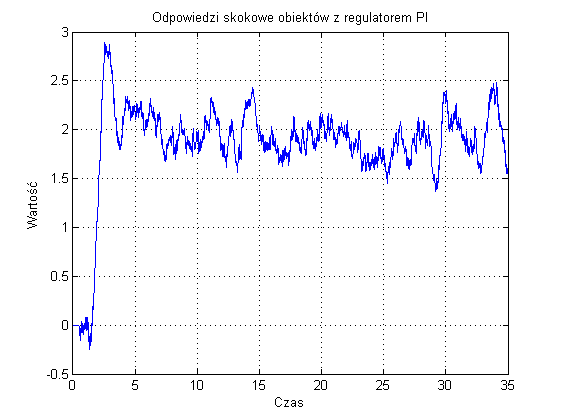
\includegraphics [width=4in]{skrypt_13.png}

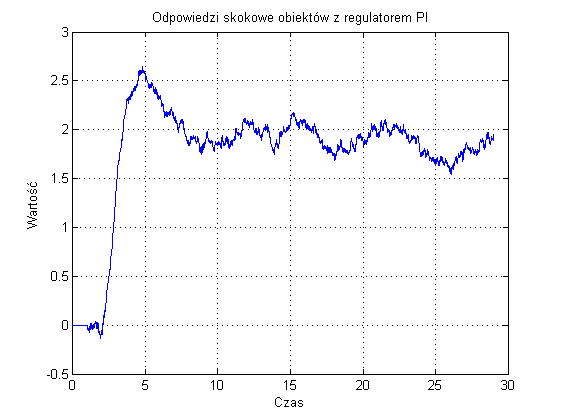
\includegraphics [width=4in]{skrypt_14.png}

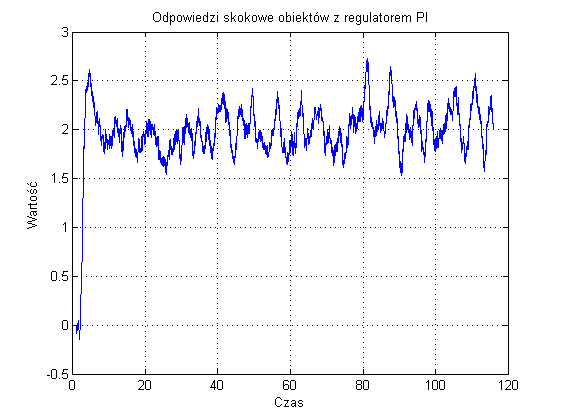
\includegraphics [width=4in]{skrypt_15.png}

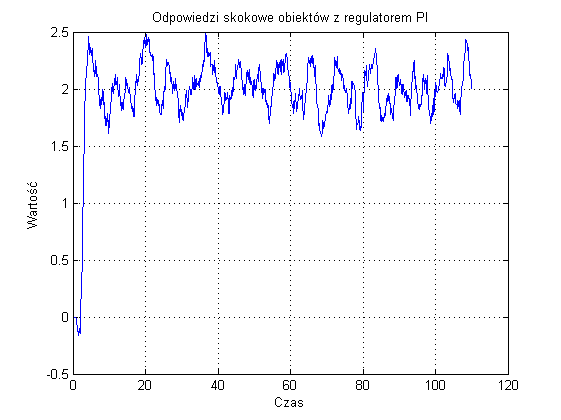
\includegraphics [width=4in]{skrypt_16.png}


\subsection*{P8}


        \color{lightgray} \begin{verbatim}Warning: When delay time is set to zero, the
transport delay block 'single_object/Transport
Delay' is automatically set to support direct
feedthrough. This may cause an algebraic loop. A
Memory Block can be used in place of the
Transport Delay to break the loop 
Warning: To use the default
trust-region-reflective algorithm you must supply
the gradient in the objective function and set
the GradObj option to 'on'. FMINCON will use the
active-set algorithm instead. For information on
applicable algorithms, see Choosing the Algorithm
in the documentation. 
Warning: Your current settings will run a
different algorithm (interior-point) in a future
release. 

Local minimum possible. Constraints satisfied.

fmincon stopped because the predicted change in the objective function
is less than the default value of the function tolerance and constraints 
are satisfied to within the default value of the constraint tolerance.



No active inequalities.
Warning: When delay time is set to zero, the
transport delay block 'single_object/Transport
Delay' is automatically set to support direct
feedthrough. This may cause an algebraic loop. A
Memory Block can be used in place of the
Transport Delay to break the loop 
Warning: To use the default
trust-region-reflective algorithm you must supply
the gradient in the objective function and set
the GradObj option to 'on'. FMINCON will use the
active-set algorithm instead. For information on
applicable algorithms, see Choosing the Algorithm
in the documentation. 
Warning: Your current settings will run a
different algorithm (interior-point) in a future
release. 
Warning: The specified delay time for
'single_object/Transport Delay' is smaller than
the step size of the fixed-step solver. This may
cause simulation results to be inaccurate.
Consider decreasing the step size of the solver
to improve accuracy 

Local minimum possible. Constraints satisfied.

fmincon stopped because the predicted change in the objective function
is less than the default value of the function tolerance and constraints 
are satisfied to within the default value of the constraint tolerance.



No active inequalities.
\end{verbatim} \color{black}
    
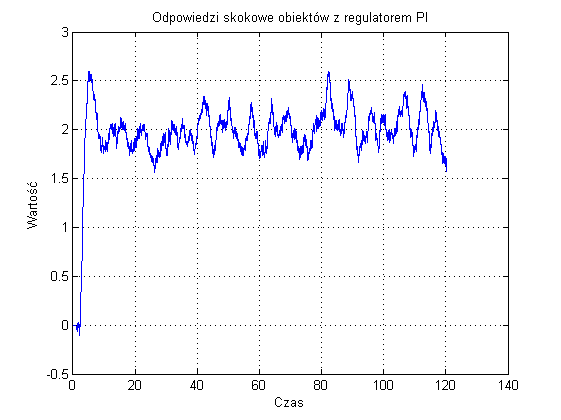
\includegraphics [width=4in]{skrypt_17.png}

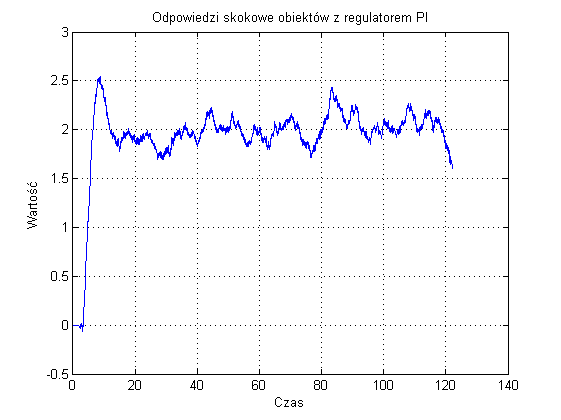
\includegraphics [width=4in]{skrypt_18.png}


\subsection*{P9}


        \color{lightgray} \begin{verbatim}Warning: When delay time is set to zero, the
transport delay block 'single_object/Transport
Delay' is automatically set to support direct
feedthrough. This may cause an algebraic loop. A
Memory Block can be used in place of the
Transport Delay to break the loop 
Warning: To use the default
trust-region-reflective algorithm you must supply
the gradient in the objective function and set
the GradObj option to 'on'. FMINCON will use the
active-set algorithm instead. For information on
applicable algorithms, see Choosing the Algorithm
in the documentation. 
Warning: Your current settings will run a
different algorithm (interior-point) in a future
release. 
Warning: The specified delay time for
'single_object/Transport Delay' is smaller than
the step size of the fixed-step solver. This may
cause simulation results to be inaccurate.
Consider decreasing the step size of the solver
to improve accuracy 

Local minimum possible. Constraints satisfied.

fmincon stopped because the predicted change in the objective function
is less than the default value of the function tolerance and constraints 
are satisfied to within the default value of the constraint tolerance.



No active inequalities.
Warning: When delay time is set to zero, the
transport delay block 'single_object/Transport
Delay' is automatically set to support direct
feedthrough. This may cause an algebraic loop. A
Memory Block can be used in place of the
Transport Delay to break the loop 
Warning: To use the default
trust-region-reflective algorithm you must supply
the gradient in the objective function and set
the GradObj option to 'on'. FMINCON will use the
active-set algorithm instead. For information on
applicable algorithms, see Choosing the Algorithm
in the documentation. 
Warning: Your current settings will run a
different algorithm (interior-point) in a future
release. 

Local minimum possible. Constraints satisfied.

fmincon stopped because the predicted change in the objective function
is less than the default value of the function tolerance and constraints 
are satisfied to within the default value of the constraint tolerance.



No active inequalities.
\end{verbatim} \color{black}
    
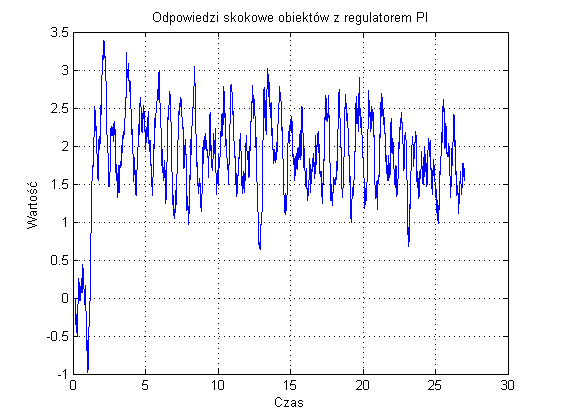
\includegraphics [width=4in]{skrypt_19.png}

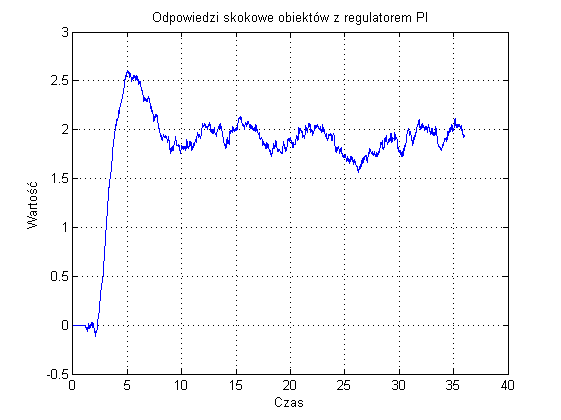
\includegraphics [width=4in]{skrypt_20.png}



\end{document}
    
